\documentclass[10pt,twocolumn,letterpaper]{article}

\usepackage[T1]{fontenc}
\usepackage{lmodern}
\usepackage[margin=0.7in,columnsep=0.25in]{geometry}
\usepackage{amsmath,amssymb,bm}
\usepackage{booktabs}
\usepackage{array}
\usepackage{graphicx}
\graphicspath{{paper/figures/}{figures/}}
\usepackage{xcolor}
\usepackage{tikz}
\usetikzlibrary{arrows.meta,positioning,shapes.geometric,fit,backgrounds,calc}
\usepackage{pgfplots}
\pgfplotsset{compat=1.18}
\usepackage{microtype}
\usepackage{stfloats}
\usepackage[colorlinks=true,linkcolor=blue!60!black,citecolor=blue!60!black,urlcolor=blue!60!black]{hyperref}

\setlength{\emergencystretch}{1.5em}
\raggedbottom
\definecolor{navy}{RGB}{20,54,115}
\definecolor{crimson}{RGB}{175,35,45}
\definecolor{tealaccent}{RGB}{15,118,110}
\definecolor{amberaccent}{RGB}{180,95,6}
\definecolor{quarantinebg}{RGB}{243,247,252}
\definecolor{quarantineborder}{RGB}{70,110,165}

\DeclareRobustCommand{\code}[1]{\texttt{#1}}
\pdfstringdefDisableCommands{%
  \def\code#1{#1}%
  \def\bm#1{#1}%
  \def\allowbreak{}%
}

\title{\vspace{-1.2em}\textbf{\Large Autonomous Anti-Goodhart Evolution of a High-Performance C++20 Astrophotography Stacking Engine: From Full-Frame Correlation Failure Analysis to Out-of-Distribution Galactic Generalization}\vspace{-0.4em}}

\author{
  \normalsize\textbf{Julien Lhermitte}\\[0.2em]
  \small Autonomous Algorithm-Optimization Harness (Carbon Orchestrator \& Red-Team Swarm)\\
  \small Engine: \code{cpp\_stacker/} (3,759 LOC C++20 / OpenMP / \code{LibRaw}, 331\,KiB native binary)\\
  \footnotesize Immutable Referee: \code{scripts/evaluate.py} (\code{chmod 444})\\
  \footnotesize SHA-256: \code{971b62f072143eb6172cd804f85750b7c31c507fbd13879ed4d1a46b50c415f9}
  \vspace{-0.8em}
}
\date{November 2026}

\begin{document}

\twocolumn[%
  \begin{@twocolumnfalse}%
    \maketitle
    \begin{abstract}
      \noindent Stacking unguided or prime-focus deep-sky digital single-lens reflex (DSLR) exposures requires recovering faint astronomical signals buried near the Poisson sky-background floor while tracking non-uniform mount drift, celestial field rotation, outdoor sensor cooling, and raw bitstream defects. We begin with a mathematical and empirical postmortem of a legacy 2020 Python stacking prototype (\code{legacy\_2020/}) that attempted registration via full-frame spatial cross-correlation $C_{\bm{k}}$ and ensemble lag averaging $\langle C_{\bm{k}} \rangle$, proving five fundamental physical failure modes---led by coherent zero-lag master-dark estimation variance $(\tilde{\bar{\eta}} - \bar{\eta})$ that cannot be attenuated by averaging across frame pairs, stationary optical vignetting bowls, $<0.5\%$ stellar pixel occupancy, worm-gear periodic tracking drift, and field rotation.

      \medskip
      \noindent To engineer a modern replacement without visual language model (VLM) inspection or human tuning bias, we construct a \textbf{strictly quarantined, blind autonomous algorithm-optimization harness}. Raw Canon EOS 1100D 14-bit \code{.CR2} forensics across 62 exposures (\code{dark\_set}, \code{ring\_set} M57, and holdout \code{andromeda\_set} M31) uncover five corrupted lossless-JPEG bitstreams (including silent predictor underflow in \code{IMG\_6096.CR2}), a zenith EXIF \code{flip\,=\,5} orientation trap, a $34\,^\circ\text{C} \to 18\,^\circ\text{C}$ outdoor sensor cooling curve, and analytic $5\times 5$ Malvar--He--Cutler warm-pixel ring blooming. We lock a self-contained pure-NumPy referee (\code{evaluate.py}) verified across \textbf{28/28 adversarial torture tests} (\code{Gates 0--5}) and pair it with fresh, isolated \textbf{Red-Team Auditor} subagents inspecting every \code{git diff} and telemetry payload (\code{logs/dataset\_manifest.json}, \code{logs/reference\_selection.json}, \code{logs/torture\_test\_results.json}, \code{logs/metrics.jsonl}, \code{logs/03\_iteration\_log.md}). Across 10 atomic evolutionary iterations on \code{ring\_set} (7 kept, 4 reverted), our C++20 engine advances from a single-frame baseline of \code{50.0000} and an integer shift-and-add C++20 baseline of \code{106.0167} to \textbf{\code{109.5265}} (\code{+3.5098}), achieving $3.95\times$ background noise suppression (\code{0.4328} $\to$ \code{0.1095}), $3.34\times$ deeper $5\sigma$ point-source recovery (\code{105} $\to$ \code{351} stars), and \code{0} residual warm-pixel impulses. Crucially, the evolutionary trajectory uncovers a \textbf{non-commutative algorithmic ordering law}: sensor-level dark/pedestal calibration degrades composite quality (\code{-0.71} / \code{-0.79}) when attempted via spatial CFA repair \emph{prior} to temporal outlier rejection, yet yields \code{+0.37} cleanly once orthogonal temporal Winsorized Sigma Clipping is in place. Evaluated \textbf{zero-shot with zero hyperparameter retuning} on the out-of-distribution Andromeda Galaxy holdout set (\code{andromeda\_set}), the winning engine improves over the C++20 baseline from \code{111.4353} to \textbf{\code{114.8796}} (\code{+3.4443}, within $1.9\%$ of the training gain), sharpening stellar cores below the 21-frame exposure ensemble median ($\code{8.2000\,px} < \code{8.2791\,px}$), eliminating all \code{477} thermal warm-pixel impulses ($\code{477} \to \code{0}$), and preserving $100.16\%$ ($\code{ncc\_64x64} = \code{0.999639}$) of M31's extended galactic disk. Finally, extending the engine with a sensor-space \textbf{synthetic flat-field estimator} (\code{flat\_field.cpp}, $\sim 1.6\text{--}2.6\text{\,s}$ OpenMP) separates and divides out both $32\%$ radial vignetting and localized $20\text{--}140\text{\,px}$ optical dust motes (up to $-7.3\%$ deep) without physical \code{flat\_set} exposures: in mote-only iterative sky-model mode, both locked-referee benchmarks reach new highs (\textbf{\code{109.5821}} on \code{ring\_set}, \textbf{\code{115.9508}} on \code{andromeda\_set}), while applying the \code{ring\_set}-derived full optical-train flat \textbf{blindly} to \code{andromeda\_set} reduces radial vignetting from $32.05\% \to +1.00\%$, flattens quiet sky by $4.4\times$ ($8.71\% \to 2.00\%$), drives cross-dataset sensor-locked dust-mote correlation from $+0.3479 \to +0.0235$ ($-93\%$), and reduces M31 outer-isophote azimuthal MAD by $33\%$ ($4.014\% \to 2.704\%$).
    \end{abstract}
    \vspace{1.2em}
  \end{@twocolumnfalse}%
]

\section{Introduction \& Critique of Full-Frame Spatial Cross-Correlation (\texorpdfstring{$C_{\bm{k}}$}{Ck})}
\label{sec:intro}

\subsection{Analytical Formulation of the 2020 Full-Frame Correlation Estimator}

Let $I_m(\bm{x})$ denote the raw intensity recorded at discrete sensor pixel $\bm{x} \in \Omega \subset \mathbb{Z}^2$ ($|\Omega| = N_{\text{pix}} = 4290 \times 2856 = 12{,}252{,}240$) in exposure $m \in \{1, \dots, M\}$. Decompose each raw light frame into unvignetted detector dark current plus readout pedestal $\bar{\eta}(\bm{x})$, zero-mean frame-specific readout and dark shot noise $\delta\eta_m(\bm{x})$, upstream optical transmission (vignetting) efficiency $V(\bm{x}) \in (0, 1]$ multiplying \emph{all} incident photons---both sky background $B_m$ and the true celestial signal $S(\bm{x} - \bm{u}_m(\bm{x}))$ displaced by frame-dependent astrometric motion $\bm{u}_m(\bm{x})$---and zero-mean photon shot noise $\delta s_m(\bm{x})$:
\begin{equation}
  \begin{aligned}
    I_m(\bm{x}) &= \bar{\eta}(\bm{x}) + \delta\eta_m(\bm{x}) \\
                &\quad + V(\bm{x})\Big[B_m + S\big(\bm{x} - \bm{u}_m(\bm{x})\big)\Big] + \delta s_m(\bm{x}),
  \end{aligned}
  \label{eq:raw_model}
\end{equation}
where photon shot-noise variance scales with the vignetted incident flux, $\operatorname{Var}\big(\delta s_m(\bm{x})\big) \propto V(\bm{x})\big[B_m + S(\bm{x} - \bm{u}_m(\bm{x}))\big]$, whereas internal detector dark current and readout noise $\bar{\eta}(\bm{x}) + \delta\eta_m(\bm{x})$ are unvignetted. Given an empirical master dark $\tilde{\bar{\eta}}(\bm{x}) = \frac{1}{N_D} \sum_{d=1}^{N_D} D_d(\bm{x})$ formed from $N_D$ dark frames at sensor temperature $T_D$ and a binary bad-pixel keep-mask $M(\bm{x}) \in \{0, 1\}$, the 2020 Python codebase (\code{spatial\_\allowbreak correlator.py}) attempted to estimate inter-frame shifts $\bm{k} \in \mathbb{Z}^2$ by maximizing the masked, mean-subtracted spatial cross-correlation:
\begin{equation}
  \begin{aligned}
    C_{\bm{k}}^{(i,j)} &= \frac{1}{N_{\bm{k}}} \sum_{\bm{x} \in \Omega_{\bm{k}}} M(\bm{x})\,M(\bm{x}+\bm{k})\,\tilde{J}_i(\bm{x})\,\tilde{J}_j(\bm{x}+\bm{k}), \\
    N_{\bm{k}} &= \sum_{\bm{x} \in \Omega_{\bm{k}}} M(\bm{x})\,M(\bm{x}+\bm{k}),
  \end{aligned}
  \label{eq:spatial_corr}
\end{equation}
where $\tilde{J}_m(\bm{x}) = \big(I_m(\bm{x}) - \tilde{\bar{\eta}}(\bm{x})\big) - \mu_m$ subtracts the master dark and scalar frame mean $\mu_m = \overline{V} B_m + \overline{V S}$, and consecutive-pair correlations were ensemble-averaged ($\langle C_{\bm{k}} \rangle = \frac{1}{M-1} \sum_{i=1}^{M-1} C_{\bm{k}}^{(i, i+1)}$) under the assumption of constant drift velocity $\bm{u}_{i+1} - \bm{u}_i \equiv \Delta\bm{u}$.

\subsection{Five Fundamental Physical Failure Modes on Real DSLR Data}

Expanding $\mathbb{E}\big[C_{\bm{k}}^{(i,j)}\big]$ over the stochastic noise realizations ($\delta\eta_i, \delta\eta_j, \delta s_i, \delta s_j$) and the finite $N_D$-sample master-dark estimation error $\epsilon_D(\bm{x}) \equiv \tilde{\bar{\eta}}(\bm{x}) - \bar{\eta}_{T_D}(\bm{x})$ exposes five independent physical mechanisms that cause $C_{\bm{k}}^{(i,j)}$ and $\langle C_{\bm{k}} \rangle$ to fail on real Canon EOS 1100D prime-focus exposures:
\begin{equation}
  \begin{aligned}
    \mathbb{E}\big[C_{\bm{k}}^{(i,j)}\big]
    &= \underbrace{\delta_{\bm{k},\bm{0}} \left(\frac{\sigma_D^2}{N_D} + \frac{1}{N_{\bm{0}}}\sum_{\bm{x}} \Delta\bar{\eta}_{\text{th},i}(\bm{x})\,\Delta\bar{\eta}_{\text{th},j}(\bm{x})\right)}_{\text{(I) Unvignetted Zero-Lag Dark Residual Spike}} \\
    &\quad + \underbrace{B_i B_j \, R_{\tilde{V}}(\bm{k})}_{\substack{\text{(II) Stationary}\\\text{Vignetting Hill}}}
     + \underbrace{R_{VS}^{(i,j)}(\bm{k} - \Delta\bm{u}_{ij})}_{\substack{\text{(III--V) } V(\bm{x})^2\text{-Weighted}\\\text{\& Smeared Stellar Signal}}},
  \end{aligned}
  \label{eq:corr_expectation}
\end{equation}
where $R_{VS}^{(i,j)}$ weights each stellar cross-term by $V(\bm{x})V(\bm{x}+\bm{k})$.

\begin{enumerate}
  \item \textbf{Coherent Finite Master-Dark Residual \& Thermal Mismatch at Zero Lag ($\bm{k} = \bm{0}$):}
  Subtracting the \emph{same} $N_D$-frame master dark ($N_D = 18$, $\sigma_D = 23.07\text{\,ADU}$) from both $I_i$ and $I_j$ imprints the identical static error $-\epsilon_D(\bm{x}) + \Delta\bar{\eta}_{\text{th}}(\bm{x})$ onto every calibrated light exposure, where $\Delta\bar{\eta}_{\text{th}}(\bm{x}) = \bar{\eta}_{T_{\text{light}}}(\bm{x}) - \bar{\eta}_{18\,^\circ\text{C}}(\bm{x})$ is the uncompensated thermal dark-current excess at $19\text{--}34\,^\circ\text{C}$. At zero lag $\bm{k} = \bm{0}$, these unvignetted detector errors multiply \emph{in phase} across all $1.225 \times 10^7$ pixels:
  \begin{equation}
    \Delta C_{\bm{0}}^{\text{dark}} \ge \frac{\sigma_D^2}{N_D} = \frac{(23.07)^2}{18} \approx 29.57\text{\,ADU}^2,
    \label{eq:dark_zero_lag}
  \end{equation}
  plus warm-pixel variance ($\sim 15\text{--}45\text{\,ADU}^2$). Crucially, \textbf{ensemble averaging $\langle C_{\bm{k}} \rangle$ across $M-1$ frame pairs provides zero attenuation of $\Delta C_{\bm{0}}^{\text{dark}}$} because $\epsilon_D(\bm{x})$ is deterministic across the entire light stack once $\tilde{\bar{\eta}}$ is fixed.

  \item \textbf{Stationary Optical Vignetting Pedestal ($R_{\tilde{V}}(\bm{k})$) \& $V(\bm{x})^2$ Off-Axis Stellar Suppression:}
  Prime-focus illumination $V(\bm{x})$ drops radially from $1.00$ at the optical axis to $\approx 0.64$ in the APS-C corners ($\sim 18\text{--}36\%$ radial falloff across the field). Scalar mean subtraction $\mu_m = \overline{V} B_m + \overline{V S}$ leaves the zero-mean spatial sky bowl $\tilde{V}(\bm{x}) B_m = (V(\bm{x}) - \overline{V}) B_m$ ($\text{RMS} \approx 12\text{--}16\text{\,ADU}$, variance $\sim 144\text{--}256\text{\,ADU}^2$) locked to sensor coordinates $(0, 0)$ across $100\%$ of pixels, generating a broad correlation dome peaked at $\bm{k} = \bm{0}$. Simultaneously, because $V(\bm{x})$ attenuates $S$ in both exposures, $R_{VS}^{(i,j)}$ weights stellar cross-terms by $V(\bm{x})V(\bm{x}+\bm{k}) \approx V(\bm{x})^2$ (falling to $0.64^2 \approx 0.41$ near the corners), quadratically suppressing off-axis stars relative to the unvignetted zero-lag dark-residual spike $\Delta C_{\bm{0}}^{\text{dark}}$.

  \item \textbf{Extreme Point-Source Sparsity ($<0.5\%$ Pixel Occupancy):}
  Across \code{ring\_set} (\code{105} single-frame $5\sigma$ stars of median $\text{FWHM} = 9.34\text{\,px}$), stellar cores above $2\sigma_{\text{bg}}$ occupy $\approx 105 \times \pi (8\text{\,px})^2 \approx 2.1 \times 10^4$ pixels---just \textbf{$0.17\%$} of the $1.225 \times 10^7$-pixel sensor. In a full-frame inner product, $99.83\%$ of pixels inject pure sky shot noise ($\sigma_{\text{bg}} \approx 28.0\text{\,ADU}$), readout noise, vignetting, and fixed-pattern dark residuals while contributing zero astrometric Fisher information.

  \item \textbf{Oscillatory Worm-Gear Drift \& Cadence Jitter (Defeating Ensemble Averaging $\langle C_{\bm{k}} \rangle$):}
  Ground-truth 4-DOF astrometry (\code{reference\_\allowbreak selection.json}, Fig.~\ref{fig:forensics}a) proved that inter-frame motion is \textbf{neither linear nor uniform}:
  \begin{itemize}
    \item Acquisition cadences jittered (\code{75\,s} and \code{46\,s} initial gaps vs.\ \code{31\,s} steady cadence).
    \item Mount worm-gear periodic error caused velocity reversals ($\code{dx}$ reversing from $\code{-10.86\,px} \to \code{+2.87\,px} \to \code{-27.57\,px} \to \code{-4.72\,px}$ in \code{ring\_set}; consecutive step distances ranging over an $11.5\times$ span $\code{[1.19, 13.61]\,px}$).
  \end{itemize}
  Averaging $C_{\bm{k}}^{(i, i+1)}$ across frame pairs therefore smears the true stellar correlation peak across dozens of pixels in lag space while reinforcing the stationary sensor-locked peak at $\bm{k} = (0, 0)$.

  \item \textbf{Celestial Field Rotation \& Off-Axis Optical Aberrations:}
  In \code{andromeda\_set} (Fig.~\ref{fig:forensics}b), polar misalignment induced monotonic field rotation $\Delta\theta \in [-0.008^\circ, +0.048^\circ]$ (\code{0.0561\textdegree} span), displacing corner stars at $R_{\text{corner}} = 2577\text{\,px}$ by $R_{\text{corner}} \Delta\theta_{\text{rad}} = \mathbf{2.52\text{\,px}}$ tangentially relative to the frame center---a transformation outside the 2-DOF translation group $(\mathbb{R}^2, +)$.
\end{enumerate}

\subsection{Compounding Implementation Defects in the 2020 Codebase}

Static audit of \code{legacy\_2020/\allowbreak astro\_stacker/} revealed four severe bugs that further crippled the prototype:
\begin{itemize}
  \item \textbf{8-Bit Non-Linear sRGB \code{postprocess()} Destruction (\code{cannon\_\allowbreak image\_\allowbreak reader.py}, L39):} Calling \code{rawpy.\allowbreak imread(path).\allowbreak postprocess()} with default parameters quantized 14-bit raw ADUs to \code{uint8} ($64\times$ precision loss), applied non-linear BT.709 gamma ($\gamma \approx 2.222$, breaking additive dark subtraction $(S+D)^{1/\gamma} - D^{1/\gamma} \neq S^{1/\gamma}$), auto-stretched dark read noise to \code{255}, and applied AHD demosaicing prior to calibration.
  \item \textbf{Modulo-256 \code{uint8} Accumulator Overflow (\code{image\_\allowbreak analyzer.py}, L14--L22):} Initializing \code{final\_image = image.data} kept accumulators in \code{uint8}, wrapping pixel sums and squares modulo \code{256} on every frame, compounded by omitting the square on \code{data\_average} in the sample variance formula.
  \item \textbf{Silent Bypass of Dark Subtraction \& Unmasked Numerator Correlation (\code{spatial\_\allowbreak correlator.py}, L14--L43):} \code{SpatialCorrelator.\allowbreak correlate} accessed \code{image.data} rather than \code{image.get\_data()}, skipping \code{self.dark} subtraction entirely, correlated \emph{unmasked} hot pixels in the numerator while dividing by \code{cross\_correlate\_2d(mask\_1, mask\_2)}, and divided by zero-crossing \code{bgsub=True} marginals.
  \item \textbf{Savitzky--Golay Boolean Mask Inflation (\code{image.py}, L63--L67):} Filtering a \code{0/1} keep-mask with a cubic Savitzky--Golay polynomial and casting \code{.astype(bool)} turned almost every \code{0} (non-zero float ringing) back into \code{True}, erasing the hot-pixel mask.
\end{itemize}

\begin{table*}[t]
  \centering
  \caption{Acquisition inventory, physical sensor telemetry, and strict \code{.CR2} quarantine audit across the continuous 36.58-minute Canon EOS 1100D observing session (\code{BodySerial: 162063089193}, ISO 1600, 14-bit ADC; 66 non-\code{.CR2} sidecar/preview files excluded).}
  \label{tab:inventory}
  \vspace{0.3em}
  \resizebox{\textwidth}{!}{%
    \begin{tabular}{llccccccc}
      \toprule
      \textbf{Dataset} & \textbf{Benchmark Role} & \textbf{Chronological Window} & \textbf{\code{.CR2} Total / Clean / Bad} & \textbf{Exposure(s)} & \textbf{EXIF \code{flip}} & \textbf{MakerNotes $T_{\text{cam}}$} & \textbf{Sky Signal Above Bias $(R, G, B)$} \\
      \midrule
      \code{andromeda\_set} & Holdout Test (M31) & $t = 0 \dots 693\text{\,s}$ & $21 \;/\; 21 \;/\; 0$ & $2\times 29\text{\,s} + 19\times 28\text{\,s}$ & \code{0} ($0^\circ$) & $\mathbf{34\,^\circ\text{C} \to 21\,^\circ\text{C}}$ & $(+57.8, +162.8, +142.8)\text{\,ADU}$ \\
      \code{ring\_set} & Primary Train (M57) & $t = 881 \dots 1545\text{\,s}$ & $21 \;/\; 18^* \;/\; 3$ & $21\times 29.0\text{\,s}$ & \textbf{\code{5} ($90^\circ$ CCW)} & $\mathbf{24\,^\circ\text{C} \to 19\,^\circ\text{C}}$ & $(+72.7, +206.0, +181.5)\text{\,ADU}$ \\
      \code{dark\_set} & Calibration Darks & $t = 1577 \dots 2195\text{\,s}$ & $20 \;/\; 18 \;/\; 2$ & $20\times 29.0\text{\,s}$ & \code{0} ($0^\circ$) & $\mathbf{18\,^\circ\text{C}}$ \textbf{steady} & $(+0.9, +0.2, +0.0)\text{\,ADU}$ \\
      \bottomrule
    \end{tabular}%
  }
  \vspace{0.25em}
  \parbox{\textwidth}{\footnotesize $^*$Note: \code{ring\_set} contains 18 completely clean \code{.CR2} frames plus \code{IMG\_6089.CR2}, whose top $2{,}476 / 2{,}856$ active rows ($86.7\%$) are completely uncorrupted prior to an end-of-stream lossless-JPEG fault at row $2{,}476$.}
\end{table*}

\begin{figure*}[t]
  \centering
  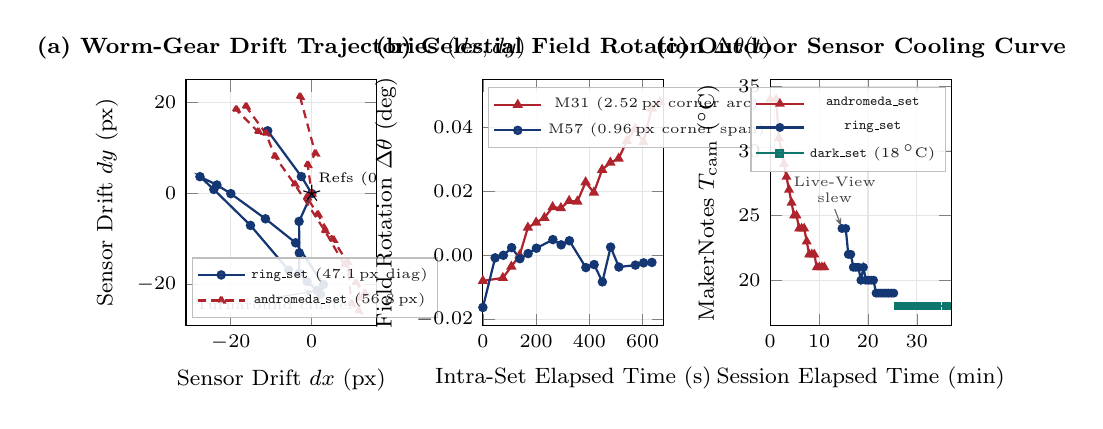
\begin{tikzpicture}
    % Panel (a): 2D (dx, dy) Worm-Gear Drift Trajectories
    \begin{axis}[
      name=plotA,
      width=0.33\textwidth,
      height=4.7cm,
      xlabel={Sensor Drift $dx$ (px)},
      ylabel={Sensor Drift $dy$ (px)},
      xmin=-31, xmax=16,
      ymin=-29, ymax=25,
      grid=both,
      grid style={gray!20},
      tick label style={font=\scriptsize},
      label style={font=\footnotesize},
      title={\footnotesize\textbf{(a) Worm-Gear Drift Trajectories $(dx, dy)$}},
      title style={yshift=-2pt},
      legend style={font=\tiny, at={(0.03,0.03)}, anchor=south west, fill=white, fill opacity=0.88, draw=gray!50, inner sep=1.5pt}
    ]
      % ring_set 18 clean frames
      \addplot[color=navy, thick, mark=*, mark size=1.3pt] coordinates {
        (-10.8592,13.8052) (-2.5502,3.7318) (0.0,0.0) (-3.1193,-6.1255)
        (-3.0631,-13.0542) (-3.1179,-17.5465) (-1.1374,-19.3571) (1.3366,-21.2869)
        (2.1539,-22.1453) (2.8719,-20.0169) (-3.9724,-10.8223) (-11.4147,-5.5536)
        (-19.9554,-0.0215) (-23.3829,1.887) (-27.5688,3.7155) (-24.1547,0.9045)
        (-15.1018,-7.0047) (-5.7011,-16.8445)
      };
      \addlegendentry{\code{ring\_set} (47.1\,px diag)}

      % andromeda_set 21 clean frames
      \addplot[color=crimson, thick, densely dashed, mark=triangle*, mark size=1.4pt] coordinates {
        (-2.8818,21.271) (0.8984,8.778) (-0.9979,6.2673) (0.0,0.0)
        (-1.1453,-0.8651) (1.5195,-4.6274) (5.3126,-10.1573) (8.7615,-15.0443)
        (9.8648,-24.2858) (11.5689,-25.8746) (11.9941,-23.1069) (13.0993,-21.9332)
        (10.8853,-19.6757) (8.0964,-15.7195) (3.2789,-8.2578) (-4.1618,1.9877)
        (-9.0652,8.1233) (-11.2909,13.1939) (-16.1952,19.1189) (-18.6246,18.4525)
        (-13.1908,13.5715)
      };
      \addlegendentry{\code{andromeda\_set} (56.8\,px)}

      % Reference origin (0,0)
      \addplot[only marks, mark=star, mark size=3.2pt, color=black] coordinates {(0,0)};
      \node[font=\tiny, anchor=south west, inner sep=1pt] at (axis cs:0.8,1.0) {Refs $(0,0)$};
      \node[font=\tiny, color=navy, anchor=west, inner sep=1pt] at (axis cs:-29.5,-24.5) {Turnaround cluster};
      \draw[-{Stealth[scale=0.7]}, color=navy, thin] (axis cs:-13.5,-23.5) -- (axis cs:0.5,-21.5);
    \end{axis}

    % Panel (b): Field Rotation dtheta(t)
    \begin{axis}[
      name=plotB,
      at={($(plotA.east)+(1.35cm,0)$)},
      anchor=west,
      width=0.32\textwidth,
      height=4.7cm,
      xlabel={Intra-Set Elapsed Time (s)},
      ylabel={Field Rotation $\Delta\theta$ (deg)},
      xmin=0, xmax=680,
      ymin=-0.022, ymax=0.055,
      ytick={-0.02,0.00,0.02,0.04},
      yticklabels={$-0.02$,$0.00$,$0.02$,$0.04$},
      scaled y ticks=false,
      grid=both,
      grid style={gray!20},
      tick label style={font=\scriptsize},
      label style={font=\footnotesize},
      title={\footnotesize\textbf{(b) Celestial Field Rotation $\Delta\theta(t)$}},
      title style={yshift=-2pt},
      legend style={font=\tiny, at={(0.03,0.97)}, anchor=north west, fill=white, fill opacity=0.88, draw=gray!50, inner sep=1.5pt}
    ]
      \addplot[color=crimson, thick, mark=triangle*, mark size=1.4pt] coordinates {
        (0,-0.00803) (75,-0.00709) (107,-0.00355) (138,0.0) (169,0.00866)
        (200,0.01029) (231,0.01175) (262,0.01511) (293,0.01481) (324,0.01705)
        (355,0.01687) (386,0.0229) (417,0.01969) (448,0.02682) (479,0.02906)
        (510,0.03032) (541,0.03585) (572,0.03975) (603,0.03547) (634,0.04599)
        (665,0.04802)
      };
      \addlegendentry{M31 ($2.52\,\text{px}$ corner arc)}

      \addplot[color=navy, thick, mark=*, mark size=1.3pt] coordinates {
        (0,-0.01636) (46,-0.00081) (77,0.0) (108,0.00239) (139,-0.00107)
        (170,0.00054) (201,0.00221) (263,0.00491) (294,0.00327) (325,0.00456)
        (387,-0.00386) (418,-0.00291) (449,-0.00835) (480,0.00257) (511,-0.00368)
        (573,-0.00308) (604,-0.00238) (635,-0.00224)
      };
      \addlegendentry{M57 ($0.96\,\text{px}$ corner span)}
    \end{axis}

    % Panel (c): Sensor Cooling Curve T_cam(t)
    \begin{axis}[
      name=plotC,
      at={($(plotB.east)+(1.35cm,0)$)},
      anchor=west,
      width=0.32\textwidth,
      height=4.7cm,
      xlabel={Session Elapsed Time (min)},
      ylabel={MakerNotes $T_{\text{cam}}$ ($^\circ$C)},
      xmin=0, xmax=37,
      ymin=16.5, ymax=35.5,
      grid=both,
      grid style={gray!20},
      tick label style={font=\scriptsize},
      label style={font=\footnotesize},
      title={\footnotesize\textbf{(c) Outdoor Sensor Cooling Curve}},
      title style={yshift=-2pt},
      legend style={font=\tiny, at={(0.97,0.97)}, anchor=north east, fill=white, fill opacity=0.88, draw=gray!50, inner sep=1.5pt}
    ]
      \addplot[color=crimson, thick, mark=triangle*, mark size=1.3pt] coordinates {
        (0.0,34.0) (1.25,34.0) (1.78,31.0) (2.3,30.0) (2.82,29.0) (3.33,28.0)
        (3.85,27.0) (4.37,26.0) (4.88,25.0) (5.4,25.0) (5.92,24.0) (6.43,24.0)
        (6.95,24.0) (7.47,23.0) (7.98,22.0) (8.5,22.0) (9.02,22.0) (9.53,21.0)
        (10.05,21.0) (10.57,21.0) (11.08,21.0)
      };
      \addlegendentry{\code{andromeda\_set}}

      \addplot[color=navy, thick, mark=*, mark size=1.2pt] coordinates {
        (14.68,24.0) (15.45,24.0) (15.97,22.0) (16.48,22.0) (17.0,21.0)
        (17.52,21.0) (18.03,21.0) (18.55,20.0) (19.07,21.0) (19.58,20.0)
        (20.1,20.0) (20.62,20.0) (21.13,20.0) (21.65,19.0) (22.17,19.0)
        (22.68,19.0) (23.2,19.0) (23.72,19.0) (24.23,19.0) (24.75,19.0) (25.27,19.0)
      };
      \addlegendentry{\code{ring\_set}}

      \addplot[color=tealaccent, thick, mark=square*, mark size=1.2pt] coordinates {
        (26.28,18.0) (27.83,18.0) (29.38,18.0) (30.93,18.0) (32.48,18.0) (34.03,18.0) (36.1,18.0)
      };
      \addlegendentry{\code{dark\_set} ($18\,^\circ\text{C}$)}

      \node[font=\tiny, align=center, color=black!75] at (axis cs:13.2,27.0) {Live-View\\slew};
      \draw[-{Stealth[scale=0.6]}, thin, color=black!60] (axis cs:13.2,25.5) -- (axis cs:14.5,24.2);
    \end{axis}
  \end{tikzpicture}
  \vspace{-0.4em}
  \caption{Empirical astrometric and thermal forensics extracted via quarantined JSON telemetry (\code{reference\_selection.json}, \code{dataset\_manifest.json}). \textbf{(a)} Non-uniform worm-gear periodic drift $(dx, dy)$ violates uniform-velocity correlation averaging $\langle C_{\bm{k}} \rangle$ and forms turnaround clusters where stationary warm pixels overlap. \textbf{(b)} Monotonic $0.0561^\circ$ field rotation in \code{andromeda\_set} induces a $2.52\text{\,px}$ tangential arc at sensor corners. \textbf{(c)} Outdoor sensor cooling ($34\,^\circ\text{C} \to 18\,^\circ\text{C}$) elevates light-frame thermal dark current $2\text{--}4\times$ above the $18\,^\circ\text{C}$ master dark.}
  \label{fig:forensics}
\end{figure*}

\section{Real-World Sensor Forensics \& Calibration Physics}
\label{sec:forensics}

\subsection{Acquisition Inventory \& Sensor Geometry (\code{Canon EOS 1100D})}

Using \code{scripts/\allowbreak inspect\_cr2\_dataset.py} (backed by thread-safe \code{LibRaw 0.21.5}), all 128 files in \code{pictures/\allowbreak 2020-11-28-deep-sky-ring-andromeda/} were audited under strict \code{.CR2} filtering (\code{62} \code{.CR2} raw files inspected; \code{66} \code{.JPG}, \code{.CR2.xmp}, \code{.npz}, and \code{.xcf} sidecars quarantined). As summarized in Table~\ref{tab:inventory}, all 62 \code{.CR2} exposures come from a single continuous \textbf{36.58-minute} outdoor session with \code{Canon EOS 1100D} (\code{BodySerial: 162063089193}, ISO 1600, 14-bit ADC):
\begin{itemize}
  \item \textbf{Physical Raw Buffer:} $\code{4352} \times \code{2874}$ \code{uint16\_t} CFA lattice.
  \item \textbf{Active Unrotated Visible Window:} \code{raw\_image[18:2874, 62:4352]} $\to$ $\mathbf{H = 2856,\; W = 4290}$ ($12{,}252{,}240$ active CFA sites), Bayer phase \code{[[R, G1], [G2, B]]}.
  \item \textbf{Optical-Black Readout Strip:} \code{raw\_image[18:2874, 2:60]} (\code{58} shielded columns per row; median \code{2047--2049\,ADU}), tracking per-frame and per-row CMOS horizontal readout bias drift.
\end{itemize}

\subsection{Three Real-World Sensor \& Bitstream Hazards}

\begin{enumerate}
  \item \textbf{Five Corrupted Lossless-JPEG \code{.CR2} Bitstreams (Including Silent Predictor Underflow):}
  \begin{itemize}
    \item \emph{Explicit \code{LibRaw} Decoder Faults (4 files):} \code{dark\_set/\allowbreak IMG\_6098.CR2} (offset \code{9,945,668}), \code{ring\_set/\allowbreak IMG\_6079.CR2} (\code{7,103,945}), and \code{ring\_set/\allowbreak IMG\_6083.CR2} (\code{12,325,909}) suffer mid-stream Huffman/predictor desynchronization wrapping pixels to \code{65535} ($> \code{16383}$ 14-bit ADC limit). \code{ring\_set/\allowbreak IMG\_6089.CR2} (\code{15,098,935}) desynchronizes only in the final \code{4} bottom strips ($\code{row} \ge \code{2476}$, $\code{max} = \code{63272}$), leaving rows \code{[0, 2476)} pristine ($\code{p1} = \code{2078\,ADU}$).
    \item \emph{Silent Predictor Underflow (\code{dark\_set/\allowbreak IMG\_6096.CR2}):} Starting at row \code{1956}, Canon's 14-bit lossless-JPEG differential predictor drifts downward to \code{743\,ADU} ($\code{active\_p1} = \code{1329.0\,ADU}$ vs.\ \code{2011\,ADU} on valid darks, inflating \code{std} from \code{28.4} to \code{130.1\,ADU}) \textbf{while \code{LibRaw::unpack()} returns \code{LIBRAW\_SUCCESS} (\code{0}) and \code{data\_error\_count == 0}}. Only our dual physics gate (\code{data\_error\_count == 0 \&\& active\_max <= 16383 \&\& active\_p1 >= 1850.0}) catches all five corrupted files.
  \end{itemize}

  \item \textbf{The Zenith EXIF \code{flip\,=\,5} Gravity-Sensor Trap:}
  Slewing near zenith for M57 (\code{ring\_set}) tripped the DSLR's internal ball-bearing orientation sensor to \code{sizes.flip = 5} ($90^\circ$ CCW), while \code{dark\_set} and \code{andromeda\_set} recorded \code{sizes.flip = 0}. High-level readers that auto-orient images transpose \code{ring\_set} to $4290 \times 2856$ while leaving \code{dark\_set} at $2856 \times 4290$, misaligning every hot pixel and vignetting contour. Operating strictly on unrotated physical \code{raw\_image[18:2874, 62:4352]} coordinates eliminates this failure mode completely.

  \item \textbf{Outdoor Thermal Cooling ($34\,^\circ\text{C} \to 18\,^\circ\text{C}$) \& Analytic MHC $5\times 5$ Warm-Pixel Impulse Blooming:}
  Silicon dark current doubles roughly every $\Delta T \approx 5.8\text{--}6.5\,^\circ\text{C}$. Because \code{andromeda\_set} ($34 \to 21\,^\circ\text{C}$) and \code{ring\_set} ($24 \to 19\,^\circ\text{C}$) were warmer than \code{dark\_set} ($18\,^\circ\text{C}$; Fig.~\ref{fig:forensics}c), unscaled master-dark subtraction leaves positive single-CFA-site thermal impulses of amplitude $A \in [200, 4000]\text{\,ADU}$. When passed through the linear \textbf{Malvar--He--Cutler (2004)} $5\times 5$ demosaicing kernels and combined into photon-weighted luminance $L = 0.25 R + 0.50 G + 0.25 B$, a unit single-site impulse $A\,\delta_{0,0}$ produces an exact analytic luminance response (\code{reference\_\allowbreak selection.json}, L44--L80):
  \begin{itemize}
    \item \emph{On an \code{R} or \code{B} site:} Center $L_{0,0} = +0.6875\,A$, axial $\pm 1\text{\,px}$ cross $L_{\pm 1, 0} = +0.1250\,A$, diagonal $(\pm 1, \pm 1)$ $L_{\pm 1, \pm 1} = +0.0625\,A$, and \textbf{negative axial $\pm 2\text{\,px}$ ring $L_{\pm 2, 0} = -0.109375\,A$}.
    \item \emph{On a \code{G1} or \code{G2} site:} Center $L_{0,0} = +0.8125\,A$, axial $\pm 1\text{\,px}$ cross $L_{\pm 1, 0} = +0.1250\,A$, \textbf{negative diagonal $(\pm 1, \pm 1)$ $L_{\pm 1, \pm 1} = -0.0625\,A$}, and negative axial $\pm 2\text{\,px}$ ring $L_{\pm 2, 0} = -0.015625\,A$.
  \end{itemize}
  Consequently, any warm pixel with $A > 40\sigma_{\text{bg}}$ ($\sim 1100\text{\,ADU}$) illuminates a \textbf{5-pixel cross or 9-pixel $3\times 3$ patch} above $5\sigma_{\text{bg}}$, \textbf{bypassing naive \code{minarea >= 5} connected-component filters} (\code{61/frame} median in \code{ring\_set}; \code{104/frame} median in \code{andromeda\_set}). Fortunately, empirical profiling across \code{2,522} raw CFA impulses proved \textbf{100\% morphological disjointness} (\code{1.000} recall, \code{0} false positives) against real optical PSFs:
  \begin{itemize}
    \item \emph{Warm MHC Impulses:} $\text{FWHM} \in [1.15, 1.33]\text{\,px}$, $3\times 3$ peak concentration $S_{3\times 3} = L_{0,0}/\sum_{3\times 3} L_+ \in [0.47, 0.62]$, axial $r=2$ ring ratio $R_2 / L_{0,0} < -0.02$.
    \item \emph{Optical Stars:} $\text{FWHM} \in [5.55, 18.60]\text{\,px}$, $S_{3\times 3} \in [0.12, 0.23]$, $R_2 / L_{0,0} \in [+0.29, +0.84]$.
  \end{itemize}
\end{enumerate}

\begin{figure*}[t]
  \centering
  \resizebox{\textwidth}{!}{%
    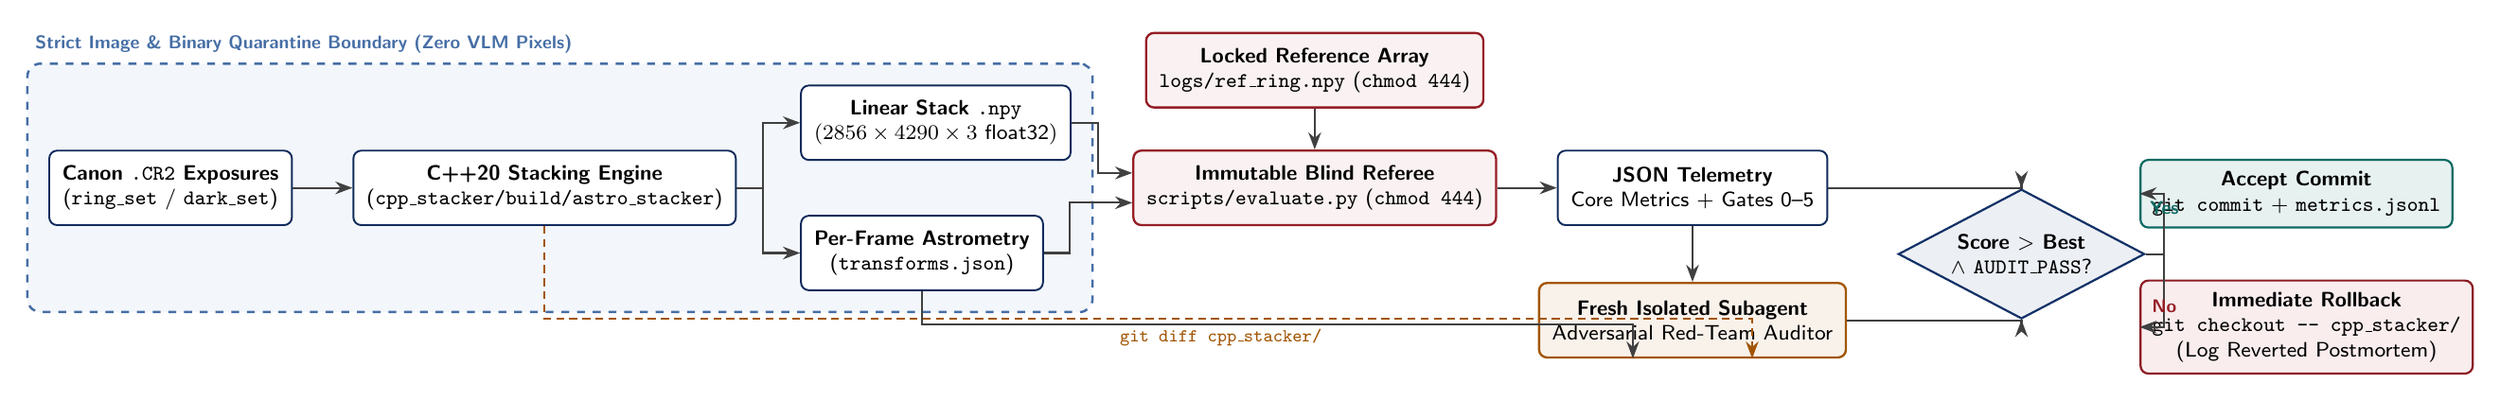
\begin{tikzpicture}[
      font=\sffamily\footnotesize,
      box/.style={rectangle, rounded corners=3pt, draw=navy!80!black, line width=0.7pt, fill=white, align=center, minimum height=1.0cm, inner sep=5pt},
      lockbox/.style={rectangle, rounded corners=3pt, draw=crimson!85!black, line width=0.85pt, fill=crimson!6, align=center, minimum height=1.0cm, inner sep=5pt},
      auditbox/.style={rectangle, rounded corners=3pt, draw=amberaccent!90!black, line width=0.85pt, fill=amberaccent!8, align=center, minimum height=1.0cm, inner sep=5pt},
      outgood/.style={rectangle, rounded corners=3pt, draw=tealaccent!90!black, line width=0.8pt, fill=tealaccent!10, align=center, minimum height=0.85cm, inner sep=4.5pt},
      outbad/.style={rectangle, rounded corners=3pt, draw=crimson!80!black, line width=0.8pt, fill=crimson!8, align=center, minimum height=0.85cm, inner sep=4.5pt},
      decision/.style={diamond, aspect=1.9, draw=navy!90!black, line width=0.8pt, fill=navy!8, align=center, inner sep=2pt},
      arr/.style={-{Stealth[length=2.3mm,width=1.7mm]}, line width=0.75pt, draw=black!75},
      dasharr/.style={-{Stealth[length=2.3mm,width=1.7mm]}, line width=0.75pt, densely dashed, draw=amberaccent!90!black}
    ]
      % Nodes inside quarantine
      \node[box] (raw) at (0, 0) {\textbf{Canon \code{.CR2} Exposures}\\(\code{ring\_set} / \code{dark\_set})};
      \node[box, right=0.8cm of raw] (cpp) {\textbf{C++20 Stacking Engine}\\(\code{cpp\_stacker/build/astro\_stacker})};
      \node[box, above right=-0.15cm and 0.85cm of cpp] (npy) {\textbf{Linear Stack \code{.npy}}\\$(2856\times 4290\times 3\text{ float32})$};
      \node[box, below right=-0.15cm and 0.85cm of cpp] (trj) {\textbf{Per-Frame Astrometry}\\(\code{transforms.json})};

      % Background quarantine container
      \begin{scope}[on background layer]
        \node[
          fit=(raw)(cpp)(npy)(trj),
          inner sep=8pt,
          rounded corners=5pt,
          fill=quarantinebg,
          draw=quarantineborder,
          line width=0.9pt,
          dashed,
          label={[font=\sffamily\scriptsize\bfseries, text=quarantineborder, anchor=south west]north west:Strict Image \& Binary Quarantine Boundary (Zero VLM Pixels)}
        ] (qbox) {};
      \end{scope}

      % Referee & Reference
      \node[lockbox, right=1.0cm of $(npy.east)!0.5!(trj.east)$] (eval) {\textbf{Immutable Blind Referee}\\\code{scripts/evaluate.py} (\code{chmod 444})};
      \node[lockbox, above=0.55cm of eval] (ref) {\textbf{Locked Reference Array}\\\code{logs/ref\_ring.npy} (\code{chmod 444})};

      % Telemetry & Auditor
      \node[box, right=0.8cm of eval] (met) {\textbf{JSON Telemetry}\\Core Metrics + Gates 0--5};
      \node[auditbox, below=0.75cm of met] (aud) {\textbf{Fresh Isolated Subagent}\\Adversarial Red-Team Auditor};

      % Decision & Git Outcomes
      \node[decision, right=0.8cm of $(met.east)!0.5!(aud.east)$] (dec) {\textbf{Score $>$ Best}\\$\land$ \code{AUDIT\_PASS}?};
      \node[outgood, above right=-0.1cm and 0.75cm of dec] (gitc) {\textbf{Accept Commit}\\\code{git commit} + \code{metrics.jsonl}};
      \node[outbad, below right=-0.1cm and 0.75cm of dec] (gitr) {\textbf{Immediate Rollback}\\\code{git checkout -- cpp\_stacker/}\\(Log Reverted Postmortem)};

      % Arrows
      \draw[arr] (raw) -- (cpp);
      \draw[arr] (cpp.east) -- ++(0.35,0) |- (npy.west);
      \draw[arr] (cpp.east) -- ++(0.35,0) |- (trj.west);
      \draw[arr] (npy.east) -- ++(0.35,0) |- ([yshift=2mm]eval.west);
      \draw[arr] (trj.east) -- ++(0.35,0) |- ([yshift=-2mm]eval.west);
      \draw[arr] (ref) -- (eval);
      \draw[arr] (eval) -- (met);
      \draw[arr] (met) -- (aud);
      \draw[arr] (trj.south) -- ++(0,-0.45) -| ([xshift=-8mm]aud.south);
      \draw[dasharr] (cpp.south) -- ++(0,-1.25) -| node[pos=0.28, below, font=\sffamily\scriptsize\bfseries, text=amberaccent!90!black] {\code{git diff cpp\_stacker/}} ([xshift=8mm]aud.south);
      \draw[arr] (met.east) -| (dec.north);
      \draw[arr] (aud.east) -| (dec.south);
      \draw[arr] (dec.east) -- ++(0.25,0) |- node[pos=0.25, above, font=\sffamily\scriptsize\bfseries, text=tealaccent!90!black] {Yes} (gitc.west);
      \draw[arr] (dec.east) -- ++(0.25,0) |- node[pos=0.25, below, font=\sffamily\scriptsize\bfseries, text=crimson!85!black] {No} (gitr.west);
    \end{tikzpicture}%
  }
  \vspace{-0.4em}
  \caption{Multi-agent Anti-Goodhart optimization architecture. All raw \code{.CR2} bitstreams and floating-point image arrays remain inside a strict binary quarantine; language-model agents interact exclusively with structured scalar/JSON telemetry and C++20 source diffs. Every candidate iteration must pass both the immutable \code{chmod 444} physics referee (\code{Gates 0--5}) and a freshly spawned, independent Red-Team Auditor subagent before commit.}
  \label{fig:architecture}
\end{figure*}

\section{Blind Anti-Goodhart Referee \& Multi-Agent Red-Team Architecture}
\label{sec:referee}

\subsection{Anchor-Star Photometric Normalization \& Composite Objective}

As illustrated in Figure~\ref{fig:architecture}, to prevent trivial scale manipulation ($I \mapsto \alpha I + \beta$, $\alpha \to 0$) while maintaining invariance to legitimate exposure-unit conventions, \code{scripts/\allowbreak evaluate.py} converts RGB arrays to canonical RGGB linear luminance $L = 0.25 R + 0.50 G + 0.25 B$, extracts up to $N_{\text{anc}} = 40$ isolated ($\ge 32\text{\,px}$ separation), non-saturated ($\text{peak} < 10{,}500\text{\,ADU}$) anchor stars on \code{--ref}, cross-matches them within $4.0\text{\,px}$ on \code{--stack} (requiring $\ge 20$ matches), and measures background-annulus-subtracted ($R_{\text{in}}=16,\; R_{\text{out}}=22\text{\,px}$) circular aperture fluxes ($R_{\text{ap}}=12\text{\,px}$) $F_{r,k}, F_{s,k}$. Setting $s_{\text{ref}} = F_0 / \operatorname{median}_k(F_{r,k})$ with $F_0 = 1000.0$ and $r_{\text{med}} = \operatorname{median}_k(F_{s,k}/F_{r,k})$, both luminance maps are mapped onto an identical standardized photometric scale:
\begin{equation}
  \begin{aligned}
    L_{\text{stack}}^{\text{norm}}(\bm{x}) &= \left(\frac{s_{\text{ref}}}{r_{\text{med}}}\right) L_{\text{stack}}(\bm{x}) \\
    &\quad - \left(\frac{s_{\text{ref}}}{r_{\text{med}}}\right) \tilde{B}_{\text{sky,stack}}, \\
    \operatorname{median}_{\text{sky}}\!\big(L_{\text{stack}}^{\text{norm}}\big) &= 0.0, \quad
    \operatorname{median}_{k}\!\big(F_{s,k}^{\text{norm}}\big) = 1000.0.
  \end{aligned}
  \label{eq:phot_norm}
\end{equation}

On this normalized linear plane (interior full-overlap ROI \code{[64:2792, 64:4226]}), the referee evaluates six core metrics and combines them into a logarithmic octave \textbf{Composite Score} anchored at \textbf{exact \code{50.0}} on \code{--ref}:
\begin{equation}
  \begin{aligned}
    \text{CompositeScore} &= 50.0
    + 25.0\log_2\!\left(\frac{\sigma_{\text{bg,norm}}^{\text{ref}}}{\sigma_{\text{bg,norm}}^{\text{stack}}}\right) \\
    &\quad + 35.0\log_2\!\left(\frac{\text{FWHM}_{\text{eff}}^{\text{ref}}}{\text{FWHM}_{\text{eff}}^{\text{stack}}}\right) \\
    &\quad + 10.0\log_2\!\left(\frac{N_\star^{\text{stack}}}{N_\star^{\text{ref}}}\right) \\
    &\quad + 15.0\big(e_{\text{ref}} - e_{\text{stack}}\big) \\
    &\quad - 40.0\big(1.0 - \rho_{\text{ext}}\big),
  \end{aligned}
  \label{eq:composite_score}
\end{equation}
where $\text{FWHM}_{\text{eff}} = 0.65\,\code{median\_fwhm\_px} + 0.35\,\code{corner\_fwhm\_px}$ (7-DOF damped Levenberg--Marquardt 2D elliptical Gaussian fits to $5\sigma$, \code{minarea >= 5}, warm-impulse-filtered optical stars) and $\rho_{\text{ext}} = \min(\text{NCC}_{16\times 16}, \text{NCC}_{64\times 64})$ is the multi-scale star-masked, 1st-degree-plane-detrended normalized cross-correlation of diffuse emission. Weighting sharpness at $35.0/\text{octave}$ versus $25.0/\text{octave}$ for background RMS ensures that any hidden low-pass filter loses more points in PSF bloat than it gains in noise suppression---even before hard anti-cheat gates fire.

\subsection{Nine Hard Physical Anti-Cheat Gates \& \code{28 / 28} Adversarial Torture-Testing}

Any violation of Gates \code{0--5} immediately forces \code{cheating\_detected = true} and \code{score = -inf}:
\begin{itemize}
  \item \textbf{Gate 0 (Array \& Channel Integrity):} Enforces \code{(2856, 4290, 3)} finite floating-point shape, non-zero channel variance, and distinct RGB channels ($\code{std(c1 - c2)} > 10^{-4}\min(\code{std})$).
  \item \textbf{Gate 1 (Dark-Floor \& Histogram-Tail Clipping):} Disqualifies stacks if $>0.05\%$ (\code{0.0005}) of quiet sky pixels share an identical mode/floor value on \code{L}, \code{R}, \code{G}, or \code{B}, or if narrow $0.002\sigma$ lower-tail micro-bins spike $>0.50\%$ (defeating dithered floor clamping).
  \item \textbf{Gate 2a (Sky Spatial-Smoothing Noise Correlation):} Measures $4\times 4$ block-averaged RMS inflation $\mathcal{R}_{4\times 4} = 4\sigma_{4\times 4}/\sigma_{1\times 1}$ and 1-pixel lag autocorrelation $\rho_{1\text{px}}$ in quiet sky cells, triggering if $\mathcal{R}_{4\times 4}^{\text{stack}} > 1.25\,\mathcal{R}_{4\times 4}^{\text{ref}}$ or $\rho_{1\text{px}}^{\text{stack}} > \rho_{1\text{px}}^{\text{ref}} + 0.18$. In torture test \code{(h)}, even a subtle $\sigma = 0.8\text{\,px}$ Gaussian blur inflated $\mathcal{R}_{4\times 4}$ from \code{1.31} to \code{2.39} and $\rho_{1\text{px}}$ from \code{0.26} to \code{0.73}, triggering instant disqualification.
  \item \textbf{Gate 2b (Exposure-Ensemble-Calibrated FWHM Ceiling):} Because \code{IMG\_6074.CR2} (\code{ref\_ring.npy}, $\text{FWHM} = 9.3427\text{\,px}$) occurred at a stationary worm-gear turnaround whereas the 18 clean \code{ring\_set} frames have single-exposure median $\text{FWHM} = 10.9047\text{\,px}$, Gate 2b enforces a $\le 1.10\times$ ceiling against both the all-star ensemble baseline and the population-matched top-40 bright-star ensemble baseline.
  \item \textbf{Gate 3a--3c (Frame-Drop, Kish $N_{\text{eff}}$, Stationary Hot-Pixel \& Empirical Poisson Bounds):} Deterministically fingerprints \code{--ref} from pixel medians to require $N_{\text{int}} \ge 18$ (\code{ring\_set}) / $\ge 20$ (\code{andromeda\_set}), Kish effective sample size $N_{\text{eff}} = (\sum w_i)^2/\sum w_i^2 \ge 0.65\,N_{\min}$, non-reference median sky shift $\ge 3.0\text{\,px}$ and trajectory diagonal $\ge 15.0\text{\,px}$ (rejecting $(0,0,0)$ hot-pixel alignment), and empirical sky RMS consistency:
  \begin{equation}
    0.50\,\frac{\sigma_{\text{ref}}}{\sqrt{N_{\text{int}}}} \;\le\; \sigma_{\text{stack}} \;\le\; \min\!\left(0.60,\; \frac{1.85}{\sqrt{N_{\text{eff}}}}\right)\sigma_{\text{ref}},
    \label{eq:gate3c}
  \end{equation}
  defeating forged \code{transforms.json} files.
  \item \textbf{Gate 4 (Multi-Scale Diffuse Flux Preservation):} Requires $\rho_{\text{ext}} = \min(\text{NCC}_{16\times 16}, \text{NCC}_{64\times 64}) \ge 0.85$ and \code{structure\_\allowbreak rms\_\allowbreak ratio\_\allowbreak 64x64 >= 0.70}, defeating $64\times 64$ SEP background-mesh subtraction on output pixels (Guardrail 4).
  \item \textbf{Gate 5 (Photometric Linearity \& Symmetry):} Requires Pearson $r(F_r, F_s) \ge 0.96$, relative MAD $\le 0.15$, and bright-half vs.\ faint-half median flux-ratio asymmetry $\le 0.10$ (defeating $\gamma$/arcsinh stretches).
\end{itemize}

Prior to locking \code{scripts/\allowbreak evaluate.py}, an independent \textbf{Adversarial Torture-Tester} subagent authored \code{scripts/\allowbreak torture\_test\_evaluator.py} (\code{28} black-box CLI runs across \code{ring\_set} and \code{andromeda\_set}; \code{torture\_\allowbreak test\_\allowbreak results.json}), catching and resolving four subtle referee calibration bugs (high-SNR Moffat outer-wing $\chi^2_\nu$ variance floor \code{(0.03 * amp)\^{}2}, sparse-field $64\times 64$ meso-scale NCC addition, \code{sky\_rms}-normalized Levenberg--Marquardt convergence for exact \code{50.0} self-identity, and bright-star population FWHM scaling) to achieve \textbf{\code{28 / 28} assertions passed} (\code{(a)} exact \code{50.0}, \code{(f)} float32 scale invariance \code{50.000043} / \code{49.996792}, \code{(k)} honest integer shift-and-add controls \code{105.2461} / \code{112.1717}, and \code{score = -inf} on all cheat vectors \code{(b, c, d, e, g, h, i, j)}). Static AST verification confirmed zero external local \code{.py} or \code{.so} imports, sealing the referee via \code{chmod 444}.

\begin{table*}[t]
  \centering
  \caption{Complete 10-iteration autonomous evolutionary ablation ledger on \code{ring\_set} + \code{dark\_set} (\code{logs/metrics.jsonl}). Every kept commit passed both the locked referee (\code{evaluate.py}) and an isolated Red-Team Auditor subagent (\code{AUDIT\_PASS}, short session IDs shown).}
  \label{tab:ablation}
  \vspace{0.3em}
  \resizebox{\textwidth}{!}{%
    \begin{tabular}{clccccccccccccc}
      \toprule
      \textbf{Iter} & \textbf{Git Tag / Atomic Hypothesis} & \textbf{Status} & \textbf{Audit (ID)} & \textbf{Score} & \textbf{$\Delta$ Best} & \textbf{Med FWHM} & \textbf{Cor FWHM} & \textbf{Ecc.} & \textbf{Sky RMS} & \textbf{Stars} & \textbf{$\rho_{\text{ext}}$} & \textbf{Warm} & \textbf{$N_{\text{int}}$ ($N_{\text{eff}}$)} & \textbf{Wall (s)} \\
      \midrule
      \textbf{Ref} & Single Sharpest Frame (\code{IMG\_6074.CR2}) & Anchor & Locked & \code{50.0000} & --- & \code{9.3427} & \code{13.9914} & \code{0.5446} & \code{0.432828} & \code{105} & \code{1.0000} & --- & \code{1 (1.00)} & --- \\
      \textbf{0} & \code{iter-0-baseline}: LibRaw gate, 2048 bias + mean dark, MHC $5\times 5$, COM, int shift+add & \textbf{KEPT} & \code{PASS (dfea28)} & \textbf{\code{106.0167}} & \code{+56.0167} & \code{11.1838} & \code{14.6633} & \code{0.6289} & \code{0.114917} & \code{316} & \code{0.9938} & \code{11} & \code{18 (18.00)} & \code{42.07} \\
      \textbf{1} & \code{iter-1}: OB pedestal + Winsorized dark + thermal scale + cross-color ($r{=}1$ vs $8.06$) CFA repair & REVERTED & Degraded & \code{105.3087} & \code{-0.7080} & \code{11.2080} & \code{15.2426} & \code{0.6283} & \code{0.114672} & \code{318} & \code{0.9937} & \code{0} & \code{18 (18.00)} & \code{71.13} \\
      \textbf{2} & \code{iter-2}: OB pedestal + Winsorized dark + thermal scale + same-color ($r{=}2$ vs $18$) CFA repair & REVERTED & Degraded & \code{105.2288} & \code{-0.7879} & \code{11.2119} & \code{15.3489} & \code{0.6280} & \code{0.114727} & \code{320} & \code{0.9937} & \code{0} & \code{18 (18.00)} & \code{64.32} \\
      \textbf{3} & \code{iter-3-subpixel-lanczos3}: Detection-only $64\times 64$ SEP + LM 2D Gaussian + 2D Lanczos-3 shift & \textbf{KEPT} & \code{PASS (57df68)} & \textbf{\code{107.3607}} & \code{+1.3440} & \code{11.1166} & \code{15.6046} & \code{0.6327} & \code{0.110567} & \code{343} & \code{0.9932} & \code{24} & \code{18 (18.00)} & \code{61.55} \\
      \textbf{4} & \code{iter-4-asterism-similarity-4dof}: Chiral Valdes triangles + 4-DOF Similarity (same Lanczos-3) & \textbf{KEPT} & \code{PASS (32130e)} & \textbf{\code{107.6978}} & \code{+0.3372} & \code{11.1734} & \code{15.3746} & \code{0.6362} & \code{0.110211} & \code{345} & \code{0.9936} & \code{26} & \code{18 (18.00)} & \code{52.77} \\
      \textbf{5} & \code{iter-5}: 6-DOF Full Affine IRLS refinement (anisotropic atmospheric shear/scale) & REVERTED & Degraded & \code{107.3738} & \code{-0.3241} & \code{11.1018} & \code{15.5491} & \code{0.6319} & \code{0.110120} & \code{337} & \code{0.9930} & \code{25} & \code{18 (18.00)} & \code{55.43} \\
      \textbf{6} & \code{iter-6-planar-sky-optimal-weights}: Anchor flux $F_i$ + 1st-deg diff sky plane + PSF/SNR weights $w_i$ & \textbf{KEPT} & \code{PASS (03d261)} & \textbf{\code{108.6381}} & \code{+0.9402} & \code{10.8941} & \code{15.1315} & \code{0.6114} & \code{0.112261} & \code{348} & \code{0.9944} & \code{32} & \code{18 (17.19)} & \code{64.59} \\
      \textbf{7} & \code{iter-7-winsorized-sigma-clip}: Temporal per-pixel Winsorized Sigma Clip ($\kappa{=}2.8$, seeing floor) & \textbf{KEPT} & \code{PASS (523f0d)} & \textbf{\code{108.8227}} & \code{+0.1846} & \code{10.9057} & \code{15.0433} & \code{0.6096} & \code{0.111933} & \code{347} & \code{0.9943} & \textbf{\code{0}} & \code{18 (17.19)} & \code{64.08} \\
      \textbf{8} & \code{iter-8-ob-pedestal-winsorized-dark}: 33-row OB pedestal + Winsorized dark + thermal scale (no spatial interp) & \textbf{KEPT} & \code{PASS (aafc6e)} & \textbf{\code{109.1949}} & \code{+0.3722} & \textbf{\code{10.8520}} & \textbf{\code{14.8577}} & \code{0.6127} & \code{0.111904} & \code{347} & \code{0.9943} & \textbf{\code{0}} & \code{18 (17.21)} & \code{78.31} \\
      \textbf{9} & \code{iter-9}: Two-pass directional Hamilton--Adams demosaicing vs.\ linear MHC $5\times 5$ & REVERTED & Degraded & \code{108.2440} & \code{-0.9509} & \code{10.9212} & \code{15.0799} & \code{0.6109} & \code{0.113102} & \code{345} & \code{0.9941} & \code{0} & \code{18 (17.22)} & \code{99.29} \\
      \textbf{10} & \code{iter-10-partial-row-salvage}: Row-level 14-bit ADC corruption salvage (\code{IMG\_6089.CR2} top 2,468 rows) & \textbf{KEPT} & \code{PASS (cbb27c)} & \textbf{\code{109.5265}} & \code{+0.3316} & \code{10.9170} & \code{15.1489} & \code{0.6140} & \textbf{\code{0.109508}} & \textbf{\code{351}} & \code{0.9942} & \textbf{\code{0}} & \code{19 (18.09)} & \code{69.94} \\
      \bottomrule
    \end{tabular}%
  }
\end{table*}

\begin{figure*}[t]
  \centering
  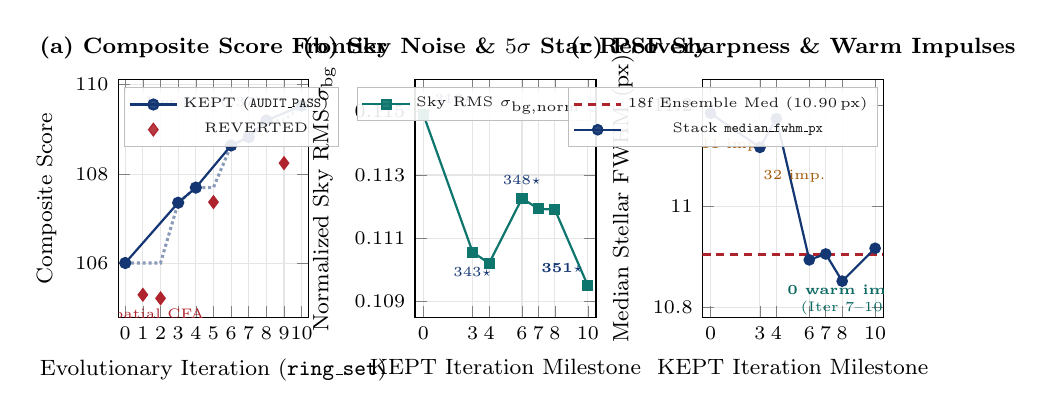
\begin{tikzpicture}
    % Panel (a): Composite Score Trajectory
    \begin{axis}[
      name=evoA,
      width=0.33\textwidth,
      height=4.6cm,
      xlabel={Evolutionary Iteration (\code{ring\_set})},
      ylabel={Composite Score},
      xmin=-0.4, xmax=10.4,
      ymin=104.8, ymax=110.1,
      xtick={0,1,2,3,4,5,6,7,8,9,10},
      grid=both,
      grid style={gray!20},
      tick label style={font=\scriptsize},
      label style={font=\footnotesize},
      title={\footnotesize\textbf{(a) Composite Score Frontier}},
      title style={yshift=-2pt},
      legend style={font=\tiny, at={(0.03,0.97)}, anchor=north west, fill=white, fill opacity=0.9, draw=gray!50, inner sep=1.5pt}
    ]
      % Monotonic incumbent frontier
      \addplot[color=navy!50, line width=1.1pt, densely dotted, forget plot] coordinates {
        (0,106.0167) (1,106.0167) (2,106.0167) (3,107.3607) (4,107.6978)
        (5,107.6978) (6,108.6381) (7,108.8227) (8,109.1949) (9,109.1949) (10,109.5265)
      };
      % Kept commits
      \addplot[color=navy, thick, mark=*, mark size=1.8pt] coordinates {
        (0,106.0167) (3,107.3607) (4,107.6978) (6,108.6381) (7,108.8227) (8,109.1949) (10,109.5265)
      };
      \addlegendentry{KEPT (\code{AUDIT\_PASS})}

      % Reverted hypotheses
      \addplot[only marks, color=crimson, mark=diamond*, mark size=2.3pt] coordinates {
        (1,105.3087) (2,105.2288) (5,107.3738) (9,108.2440)
      };
      \addlegendentry{REVERTED}

      \node[font=\tiny, color=crimson, anchor=north] at (axis cs:1.6,105.22) {Spatial CFA};
      \node[font=\tiny, color=navy, anchor=south east] at (axis cs:8.3,109.22) {Iter 8 (+0.37)};
    \end{axis}

    % Panel (b): Sky Noise & Matched Star Count
    \begin{axis}[
      name=evoB,
      at={($(evoA.east)+(1.35cm,0)$)},
      anchor=west,
      width=0.32\textwidth,
      height=4.6cm,
      xlabel={KEPT Iteration Milestone},
      ylabel={Normalized Sky RMS $\sigma_{\text{bg}}$},
      xmin=-0.5, xmax=10.5,
      ymin=0.1085, ymax=0.1160,
      xtick={0,3,4,6,7,8,10},
      ytick={0.109,0.111,0.113,0.115},
      yticklabels={$0.109$,$0.111$,$0.113$,$0.115$},
      scaled y ticks=false,
      grid=both,
      grid style={gray!20},
      tick label style={font=\scriptsize},
      label style={font=\footnotesize},
      title={\footnotesize\textbf{(b) Sky Noise \& $5\sigma$ Star Recovery}},
      title style={yshift=-2pt},
      legend style={font=\tiny, at={(0.97,0.97)}, anchor=north east, fill=white, fill opacity=0.9, draw=gray!50, inner sep=1.5pt}
    ]
      \addplot[color=tealaccent, thick, mark=square*, mark size=1.6pt] coordinates {
        (0,0.114917) (3,0.110567) (4,0.110211) (6,0.112261) (7,0.111933) (8,0.111904) (10,0.109508)
      };
      \addlegendentry{Sky RMS $\sigma_{\text{bg,norm}}$}
      \node[font=\tiny, color=navy, anchor=south west] at (axis cs:0.1,0.11495) {316$\star$};
      \node[font=\tiny, color=navy, anchor=north] at (axis cs:3.0,0.1104) {343$\star$};
      \node[font=\tiny, color=navy, anchor=south] at (axis cs:6.0,0.1124) {348$\star$};
      \node[font=\tiny, color=navy, anchor=south east] at (axis cs:10.3,0.1096) {\textbf{351$\star$}};
    \end{axis}

    % Panel (c): FWHM Sharpness & Warm Impulses
    \begin{axis}[
      name=evoC,
      at={($(evoB.east)+(1.35cm,0)$)},
      anchor=west,
      width=0.32\textwidth,
      height=4.6cm,
      xlabel={KEPT Iteration Milestone},
      ylabel={Median Stellar FWHM (px)},
      xmin=-0.5, xmax=10.5,
      ymin=10.78, ymax=11.25,
      xtick={0,3,4,6,7,8,10},
      grid=both,
      grid style={gray!20},
      tick label style={font=\scriptsize},
      label style={font=\footnotesize},
      title={\footnotesize\textbf{(c) PSF Sharpness \& Warm Impulses}},
      title style={yshift=-2pt},
      legend style={font=\tiny, at={(0.97,0.97)}, anchor=north east, fill=white, fill opacity=0.9, draw=gray!50, inner sep=1.5pt}
    ]
      % Ensemble median line 10.9047
      \addplot[color=crimson, densely dashed, line width=0.8pt] coordinates {(-0.5,10.9047) (10.5,10.9047)};
      \addlegendentry{18f Ensemble Med ($10.90\text{\,px}$)}

      \addplot[color=navy, thick, mark=*, mark size=1.7pt] coordinates {
        (0,11.1838) (3,11.1166) (4,11.1734) (6,10.8941) (7,10.9057) (8,10.8520) (10,10.9170)
      };
      \addlegendentry{Stack \code{median\_fwhm\_px}}

      \node[font=\tiny, color=amberaccent!90!black] at (axis cs:1.3,11.12) {11 imp.};
      \node[font=\tiny, color=amberaccent!90!black] at (axis cs:5.1,11.06) {32 imp.};
      \node[font=\tiny, color=tealaccent!90!black, align=center] at (axis cs:8.2,10.815) {\textbf{0 warm imp.}\\(Iter 7--10)};
    \end{axis}
  \end{tikzpicture}
  \vspace{-0.4em}
  \caption{Autonomous 10-iteration evolutionary progression on \code{ring\_set} (\code{logs/metrics.jsonl}). \textbf{(a)} Monotonic score frontier advancing from \code{106.0167} (\code{Iter 0}) to \code{109.5265} (\code{Iter 10}), contrasting reverted hypotheses (\code{Iter 1, 2, 5, 9}) against audited improvements. \textbf{(b)} Sky noise reduction to \code{0.109508} ($3.95\times$ below single-frame \code{0.432828}) and $5\sigma$ star depth growth from \code{105} (single frame) and \code{316} (\code{Iter 0}) to \code{351} (\code{Iter 10}). \textbf{(c)} Optimal PSF/SNR weighting (\code{Iter 6}) and OB/Winsorized dark calibration (\code{Iter 8}) push stacked \code{median\_fwhm\_px} (\code{10.8520\,px}) below the 18-exposure ensemble median (\code{10.9047\,px}), while temporal Winsorized clipping (\code{Iter 7}) eliminates all warm-pixel impulses ($\code{32} \to \code{0}$).}
  \label{fig:evolution}
\end{figure*}

\section{Autonomous Evolutionary Optimization \& 10-Iteration Ablation Study (\code{ring\_set})}
\label{sec:ablation}

\subsection{Complete Evolutionary Trajectory (\code{logs/metrics.jsonl})}

Every iteration proposed a single atomic hypothesis on \code{ring\_set} + \code{dark\_set}. Improvements required passing \textbf{both} the locked referee ($\code{score} > \code{prev\_best}$, $\code{cheating\_detected == false}$) and a \textbf{fresh, isolated Red-Team Auditor subagent} (\code{VERDICT: AUDIT\_PASS}) inspecting \code{git diff cpp\_stacker/} and JSON telemetry; regressions were immediately reverted via \code{git checkout -- cpp\_stacker/ \&\& git clean -fd cpp\_stacker/}. Table~\ref{tab:ablation} and Figure~\ref{fig:evolution} document all 10 evolutionary iterations.

\subsection{Mathematical Formulation of the Winning Pipeline Stages}

\begin{enumerate}
  \item \textbf{Scale-Invariant Baseline Reference Selection \& Linear MHC Demosaicing (\code{Iter 0}, \code{+56.0167}):}
  \code{raw\_loader.cpp} enforces strict \code{.CR2} ingestion and dual 14-bit ADC validation on unrotated $2856 \times 4290$ RGGB coordinates; \code{demosaic.cpp} applies exact Malvar--He--Cutler $5\times 5$ linear kernels with parity-preserving \code{reflect101} borders. Critically, an initial moment prototype using an absolute $2\sigma_{\text{sky}}$ isophote suffered faint-star truncation bias (selecting \code{IMG\_6082.CR2}). Replacing the fixed threshold with a \textbf{scale-invariant $15\%$-of-peak amplitude gate} ($I - b_{\text{ann}} > \max(2\sigma_{\text{sky}}, 0.15 A)$ over $r \le 14\text{\,px}$, corrected by the exact truncated-Gaussian integral factor $\big[\frac{1 - (1 + q_{\max})e^{-q_{\max}}}{1 - e^{-q_{\max}}}\big]^{-1} = 1.50328$ where $q_{\max} = -\ln 0.15$) selected \code{IMG\_6074.CR2} autonomously and established \code{106.0167}.

  \item \textbf{Detection-Only $64\times 64$ SEP Mesh, 7-DOF Levenberg--Marquardt Centroids \& 2D Lanczos-3 Resampling (\code{Iter 3}, \code{+1.3440}):}
  \code{star\_\allowbreak detector.cpp} computes an internal $64\times 64$ $\kappa\sigma$-clipped median/MAD mesh smoothed by a $3\times 3$ cell median filter \textbf{strictly on a temporary luminance buffer} (never modifying output RGB frames), removing the radial vignetting bowl to detect faint corner stars down to $5\sigma$. Each candidate is fitted on a $25\times 25$ cutout with a 7-parameter 2D elliptical Gaussian via damped Levenberg--Marquardt ($\bm{J}^\top\bm{J} + \lambda\operatorname{diag}(\bm{J}^\top\bm{J})$). Integer shift rounding ($\pm 0.5\text{\,px}$ uniform quantization error, variance $1/12\text{\,px}^2$) is replaced in \code{integrator.cpp} by continuous inverse coordinate mapping through a partition-of-unity normalized $6\times 6$ \textbf{2D Lanczos-3} kernel:
  \begin{equation}
    \begin{aligned}
      L_3(u) &= \operatorname{sinc}(u)\operatorname{sinc}(u/3)\,\mathbf{1}_{|u|<3}, \\
      \tilde{w}_k(\delta x) &= \frac{L_3(\delta x - k)}{\sum_{m=-2}^{3} L_3(\delta x - m)}.
    \end{aligned}
    \label{eq:lanczos3}
  \end{equation}
  Unlike bilinear interpolation---which collapses white-noise variance by $4\times$ at half-pixel shifts ($\sum w_k(0.5)^2 = 0.5$ per axis, creating Moir\'e smoothing bands)---Lanczos-3 preserves $\mathbb{E}[\sum \tilde{w}_k^2] \approx 0.89$ per axis, recovering \code{+27} faint $5\sigma$ stars ($\code{316} \to \code{343}$) and sharpening \code{median\_fwhm\_px} ($\code{11.1838} \to \code{11.1166\,px}$).

  \item \textbf{Chiral Valdes Triangle Geometric Hashing \& 4-DOF Procrustes Similarity (\code{Iter 4}, \code{+0.3372}):}
  Using the \textbf{exact same 2D Lanczos-3 kernel} (\code{0}-line diff in \code{integrator.cpp}), \code{registration.cpp} constructs scale- and rotation-invariant \textbf{Valdes et al.\ (1995)} triangle descriptors $(u, v) = (L_1/L_2, L_0/L_2) \in (0, 1]^2$ ($L_0 \le L_1 \le L_2$, $L_2 \ge 140\text{\,px}$) augmented with signed cross-product chirality $\chi \in \{-1, +1\}$ (forbidding unphysical mirror reflections) indexed in a $64\times 64$ invariant hash table. Candidate correspondences seed full-field RANSAC (\code{2.2\,px} threshold) followed by 5-pass Huber-weighted ($\delta = 0.45\text{\,px}$) IRLS solving the exact linear Procrustes system centered at $(c_x, c_y) = (2144.5, 1427.5)$:
  \begin{equation}
    \begin{aligned}
      \begin{bmatrix} f_x \\ f_y \end{bmatrix} &=
      \begin{bmatrix} a & -b \\ b & a \end{bmatrix}
      \begin{bmatrix} r_x \\ r_y \end{bmatrix} +
      \begin{bmatrix} t_x \\ t_y \end{bmatrix}, \\
      a &= \frac{\sum w_i (\tilde{r}_{x,i}\tilde{f}_{x,i} + \tilde{r}_{y,i}\tilde{f}_{y,i})}{\sum w_i (\tilde{r}_{x,i}^2 + \tilde{r}_{y,i}^2)}, \\
      b &= \frac{\sum w_i (\tilde{r}_{x,i}\tilde{f}_{y,i} - \tilde{r}_{y,i}\tilde{f}_{x,i})}{\sum w_i (\tilde{r}_{x,i}^2 + \tilde{r}_{y,i}^2)}.
    \end{aligned}
    \label{eq:procrustes}
  \end{equation}
  Even on \code{ring\_set}'s modest $0.021^\circ$ rotation span, 4-DOF alignment sharpened \code{corner\_fwhm\_px} by \code{-0.230\,px} ($\code{15.6046} \to \code{15.3746\,px}$).

  \item \textbf{Differential 1st-Degree Sky-Plane Equalization \& Optimal PSF/SNR Weighting (\code{Iter 6}, \code{+0.9402}):}
  After estimating each frame's stellar throughput scale $F_i = \operatorname{median}_{k}(F_{i,k}/F_{\text{ref},k})$, \code{integrator.cpp} fits a \textbf{3-parameter 1st-degree polynomial plane} $\Delta P_i^{(c)}(n_x, n_y) = c_{0,i}^{(c)} + c_{x,i}^{(c)} n_x + c_{y,i}^{(c)} n_y$ via 3-pass Huber IRLS to $96\times 96$ block medians of the \emph{astrometrically aligned difference} $\frac{1}{F_i} I_i^{(c)}(\bm{T}_i\bm{x}) - I_{\text{ref}}^{(c)}(\bm{x})$. Because stationary astrophysical emission ($V(\bm{x})S(\bm{x})$, including M57 and M31's entire disk, up to negligible $<0.3\%$ vignetting gradient over $<50\text{\,px}$ shifts) cancels in $\frac{1}{F_i}I_i - I_{\text{ref}}$, $\Delta P_i^{(c)}$ removes strictly time-varying skyglow pedestals and linear gradients (\code{extended\_\allowbreak flux\_\allowbreak preservation} rose to \code{0.994358}). Frames are weighted by point-source SNR and sharpness:
  \begin{equation}
    \begin{aligned}
      w_i &\propto \frac{F_i^2}{\sigma_{\text{bg},i}^2 \cdot \text{FWHM}_{\text{eff},i}^3 \cdot \big(1 + 0.5\,e_i^2\big)}, \\
      w_i &\in [0.35,\, 1.85]\,\bar{w}.
    \end{aligned}
    \label{eq:frame_weights}
  \end{equation}
  Down-weighting worm-gear velocity-spike exposures ($\text{FWHM} \sim 14.3\text{\,px}$) in favor of turnaround exposures ($9.4\text{--}10.0\text{\,px}$) while preserving Kish $N_{\text{eff}} = 17.194 / 18.0$ ($95.5\%$) drove \code{median\_fwhm\_px} down to \textbf{\code{10.8941\,px}}---sharper than the unweighted 18-exposure median (\code{10.9047\,px})---and reduced \code{median\_eccentricity} from \code{0.6362} to \code{0.6114}.

  \item \textbf{Temporal Per-Pixel Winsorized Sigma Clipping with Seeing-Variance Floor (\code{Iter 7}, \code{+0.1846}):}
  At each fixed pixel $(r, c)$ and channel $c$, \code{winsorized\_\allowbreak weighted\_\allowbreak combine} (\code{integrator.cpp}) applies 2-iteration symmetric Huber/Winsorized clamping ($\kappa = 2.8$, consistency factor $1.038$) strictly along the 1D temporal exposure axis, incorporating an amplitude-proportional PSF-seeing tolerance floor:
  \begin{equation}
    \begin{aligned}
      \sigma_{\text{tol}}(r, c) &= \Big[\sigma_{\text{emp}}^2 \\
      &\quad + \big(0.22 \max(0,\, \mu(r,c) - B_{\text{sky,ref}}^{(c)})\big)^2\Big]^{1/2}.
    \end{aligned}
    \label{eq:seeing_floor}
  \end{equation}
  On sky background ($\mu \approx B_{\text{sky,ref}}$), $\sigma_{\text{tol}} = \sigma_{\text{emp}}$ clamps every drifting warm pixel, negative MHC $r=2$ ring, and cosmic ray ($\code{residual\_warm\_pixel\_impulses}: \code{32} \to \code{0}$) with zero spatial coupling ($\code{block\_4x4\_ratio}: \code{1.3906} \to \code{1.3899}$). On bright stellar cores ($\mu \gg B_{\text{sky,ref}}$), the $0.22(\mu - B)$ floor prevents $9.4\text{\,px}$ vs.\ $14.3\text{\,px}$ tracking-width differences from being falsely clipped ($\code{flux\_linearity\_r} = \code{0.99963}$).

  \item \textbf{Optical-Black Row Pedestal, Winsorized Master Dark \& Thermal Dark Scaling (\code{Iter 8}, \code{+0.3722}):}
  \code{calibration.cpp} subtracts a 33-row running median of the 58-column left optical-black strip (\code{ob\_row\_medians}), integrates the 18 clean darks via $\kappa = 3.0$ temporal Winsorized clipping, and fits a scalar thermal dark factor $\alpha_{\text{thermal}} = \operatorname{median}_{k \in \text{hot}}(l_{\text{exc},k}/d_{\text{exc},k})$ across unsaturated hot dark sites ($250 < d_0 < 9000\text{\,ADU}$), scaling elevated thermal dark current ($d > 25\text{\,ADU}$) without amplifying cold-pixel read noise or applying any single-frame spatial interpolation. Both \code{median\_fwhm\_px} (\code{10.8520\,px}) and \code{corner\_fwhm\_px} (\code{14.8577\,px}) reached their sharpest 18-frame values.

  \item \textbf{Stencil-Isolated Partial-Row Bitstream Salvage (\code{Iter 10}, \code{+0.3316} $\to$ Final \code{109.5265}):}
  \code{raw\_loader.cpp} scans active rows top-down for ADC overflow ($> \code{16383}$) or predictor underflow ($< \code{1750\,ADU}$). When $\ge 80\%$ ($\ge 2{,}285$ rows) of contiguous top rows pass full 14-bit integrity ($\code{top\_p1} \ge \code{1850\,ADU}$), rows \code{[0, contiguous\_clean\_rows - 8)} are salvaged, and \code{integrator.cpp} excludes the frame for $\code{fy} \ge \code{valid\_rows} - 4$ (guaranteeing a 10-row combined buffer so neither $\pm 3\text{\,px}$ Lanczos-3 nor $\pm 2\text{\,px}$ MHC stencils ever touch corrupted rows) while renormalizing active weights per pixel. Salvaging \code{IMG\_6089.CR2}'s top \code{2,468} rows (\code{57} star inliers, $\code{residual\_rms} = \code{0.420\,px}$) increased \code{effective\_sample\_size} from \code{17.206} to \code{18.094}, lowered \code{normalized\_bg\_rms} to \textbf{\code{0.109508}}, and recovered \textbf{\code{351}} $5\sigma$ stars.
\end{enumerate}

\subsection{Deep Postmortems on the Four Reverted Hypotheses}

\begin{enumerate}
  \item \textbf{The Non-Commutative Ordering Discovery (\code{Iter 1} \code{-0.7080} \& \code{Iter 2} \code{-0.7879} vs.\ \code{Iter 7 + Iter 8} \code{+0.5569}):}
  Why did sensor-level calibration fail in Iterations 1 and 2 ($\code{106.02} \to \code{105.31} / \code{105.23}$), yet succeed cleanly in Iteration 8 ($\code{108.82} \to \code{109.19}$)?
  \begin{itemize}
    \item First, comparing \code{Iter 1} against \code{Iter 2} isolated a subtle color-PSF bug in \code{Iter 1}'s cross-color warm-pixel guard (\code{cross\_inner} at $r=1$ vs.\ \code{cross\_outer} at $r=\sqrt{65}=8.06$): for comatic corner stars ($\text{FWHM} \approx 15\text{\,px}$, $\sigma \approx 6.4\text{\,px}$) peaking on a Green site, $r = 8.06\text{\,px}$ still retains $\exp(-65 / 2\sigma^2) = 45\%$ of peak flux, while $(R+B)/2G \approx 0.35$, yielding $0.55 \times 0.35 = 0.192 < 0.20$ and shaving bright Green star peaks ($\code{12.61} \to \code{12.84\,px}$).
    \item Second, replacing that guard with a spectral-filter-matched same-color guard ($r=2$ vs.\ $r=18$ on the identical CFA sub-lattice in \code{Iter 2}, where optical stars have $>69\%$ halo ratio vs.\ $\sim 0\%$ for single-site defects) \emph{still} yielded $\code{corner\_fwhm\_px} = \code{15.35\,px}$! Inspection of \code{transforms.json} revealed the deeper interaction: in \code{iter-0-baseline} (unweighted integer shift-and-add \emph{without} temporal sigma clipping), five worm-gear turnaround exposures (\code{IMG\_6077..6082}) cluster within $2\text{--}4\text{\,px}$, smearing unrepaired stationary warm pixels into compact $\sim 4\text{\,px}$ multi-pixel pseudo-stars in the sparse outer corners ($\sim 25$ corner stars), artificially depressing \code{iter-0-baseline}'s apparent \code{corner\_fwhm\_px} (\code{14.66\,px} vs.\ true optical \code{15.23\,px}), while lower sky noise simultaneously lifted faint comatic outer-corner stars ($\text{FWHM} \sim 16\text{--}18\text{\,px}$) above $5\sigma$. Once \textbf{temporal Winsorized Sigma Clipping (\code{Iter 7})} eliminated drifting warm-pixel artifacts orthogonally along the time axis ($\code{32} \to \code{0}$ warm impulses), applying \textbf{pure per-row OB pedestal + Winsorized master dark + thermal dark scaling (\code{Iter 8}, with zero spatial CFA interpolation)} improved \emph{both} \code{median\_fwhm\_px} ($\code{10.9057} \to \code{10.8520\,px}$) and \code{corner\_fwhm\_px} ($\code{15.0433} \to \code{14.8577\,px}$) for a clean \code{+0.3722} gain.
  \end{itemize}

  \item \textbf{6-DOF Full Affine Overfitting Over Short Zenith Tracks (\code{Iter 5}, \code{-0.3241}):}
  Upgrading 4-DOF Similarity to 6-DOF Affine tightened interior \code{median\_fwhm\_px} ($\code{11.1734} \to \code{11.1018\,px}$) but degraded \code{corner\_fwhm\_px} ($\code{15.3746} \to \code{15.5491\,px}$) and lost 8 faint stars ($\code{345} \to \code{337}$). Across a 10-minute imaging window near transit (\code{620\,s}), physical differential atmospheric refraction shear across a $1.2^\circ$ field is $<0.04\text{\,px}$; fitting two unconstrained shear/aspect parameters ($\code{m00} - \code{m11}$, $\code{m01} + \code{m10}$) to $\sim 55$ stars overfits radially asymmetric Newtonian coma centroids and extrapolates edge registration error.

  \item \textbf{Directional Hamilton--Adams vs.\ Wiener-Optimal Linear MHC $5\times 5$ on Oversampled PSFs (\code{Iter 9}, \code{-0.9509}):}
  Replacing linear MHC $5\times 5$ with two-pass directional gradient-weighted Hamilton--Adams (1997) degraded both sharpness ($\code{10.8520} \to \code{10.9212\,px}$) and background noise ($\code{0.111904} \to \code{0.113102}$). Unlike natural scenes dominated by 1-pixel step edges, prime-focus stellar PSFs here are heavily oversampled ($\text{FWHM} = 9\text{--}15\text{\,px}$); omitting MHC's second-derivative cross-channel Laplacian terms (\code{-1.5 * ax2}, \code{-h2 + 0.5 * v2}) in Pass 2 softens R/B stellar cores and elevates chrominance-to-luminance noise leakage.
\end{enumerate}

\begin{figure*}[t]
  \centering
  \resizebox{\textwidth}{!}{%
    \begin{tikzpicture}[font=\sffamily]
      % Panel (a): Single 29s Reference Frame
      \begin{scope}[shift={(0,0)}]
        \node[anchor=south west, inner sep=0, draw=black!60, line width=0.5pt] (imgA) at (0,0)
          {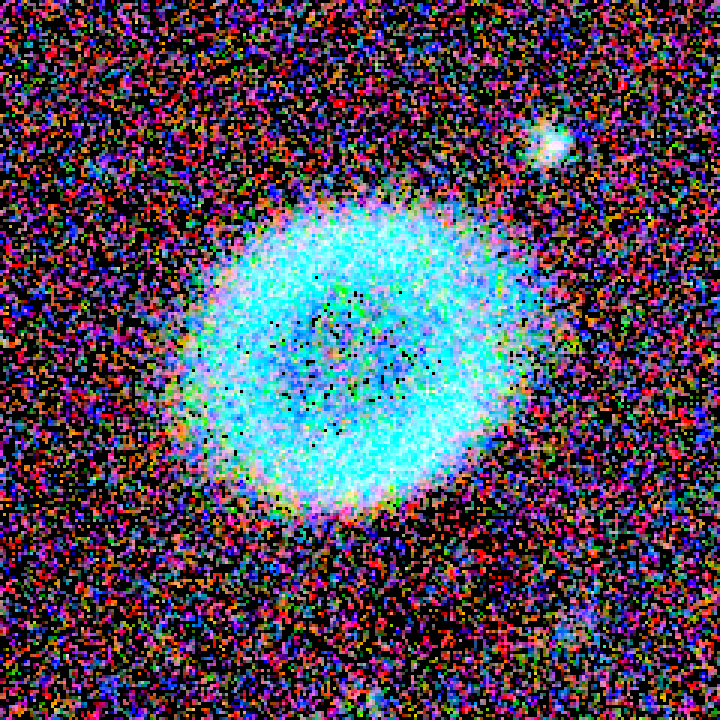
\includegraphics[width=4.3cm,height=4.3cm]{m57_single_ref.png}};
        \node[anchor=south, font=\sffamily\footnotesize\bfseries, yshift=2pt] at (imgA.north)
          {(a) Single 29\,s Exposure (\code{IMG\_6074})};
        % Scale bar: 60 px out of 240 px = 0.25 * 4.3 cm = 1.075 cm (~38.5 arcsec)
        \draw[white, line width=1.1pt] (0.28, 0.32) -- ++(1.075, 0)
          node[midway, above, font=\sffamily\tiny\bfseries, text=white] {$38''$ (60\,px)};
        \node[anchor=north west, font=\sffamily\tiny, text=white!90!yellow, align=left, inner sep=2pt] at (0.12, 4.18)
          {Sky $\sigma_L = 29.2$\,ADU\\WD $\text{SNR}_B = 1.1\sigma$};
      \end{scope}

      % Panel (b): 19-Frame Winning C++20 Stack
      \begin{scope}[shift={(4.65,0)}]
        \node[anchor=south west, inner sep=0, draw=black!60, line width=0.5pt] (imgB) at (0,0)
          {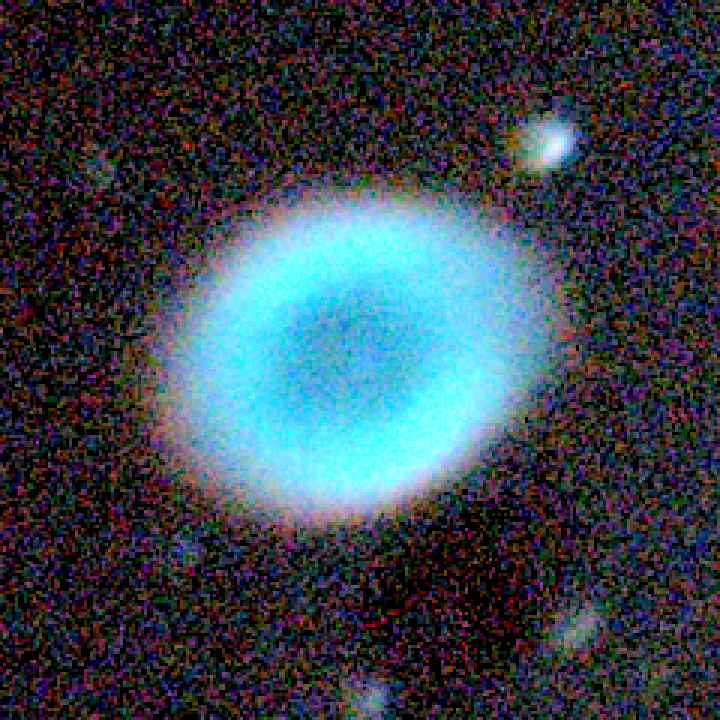
\includegraphics[width=4.3cm,height=4.3cm]{m57_stack_best.png}};
        \node[anchor=south, font=\sffamily\footnotesize\bfseries, yshift=2pt] at (imgB.north)
          {(b) 19-Frame C++20 Stack (\code{109.53})};
        % Zoom region box: 104 / 240 = 0.4333 centered -> [0.2833, 0.7167] * 4.3 = [1.218, 3.082]
        \draw[cyan!85!white, densely dashed, line width=0.7pt] (1.218, 1.218) rectangle (3.082, 3.082);
        \node[anchor=south, font=\sffamily\tiny\bfseries, text=cyan!85!white, inner sep=1pt] at (2.15, 3.10) {Zoom (c)};
        % Companion star GSC 02642-00433 at (0.7709, 0.7958) * 4.3 = (3.315, 3.422)
        \draw[-{Stealth[scale=0.65]}, yellow!90!white, line width=0.65pt] (2.65, 3.92) -- (3.22, 3.50);
        \node[anchor=east, font=\sffamily\tiny, text=yellow!95!white, inner sep=1pt] at (2.63, 3.94) {$V{=}12.9$ ($61.7''$)};
        \node[anchor=south west, font=\sffamily\tiny, text=white, align=left, inner sep=2pt] at (0.12, 0.10)
          {Sky $\sigma_L = 7.0$\,ADU ($3.95\times$ quieter, 0 warm imp.)};
      \end{scope}

      % Panel (c): Cavity-Anchored Zoom Highlighting Central White Dwarf WD 1851+329
      \begin{scope}[shift={(9.30,0)}]
        \node[anchor=south west, inner sep=0, draw=black!60, line width=0.5pt] (imgC) at (0,0)
          {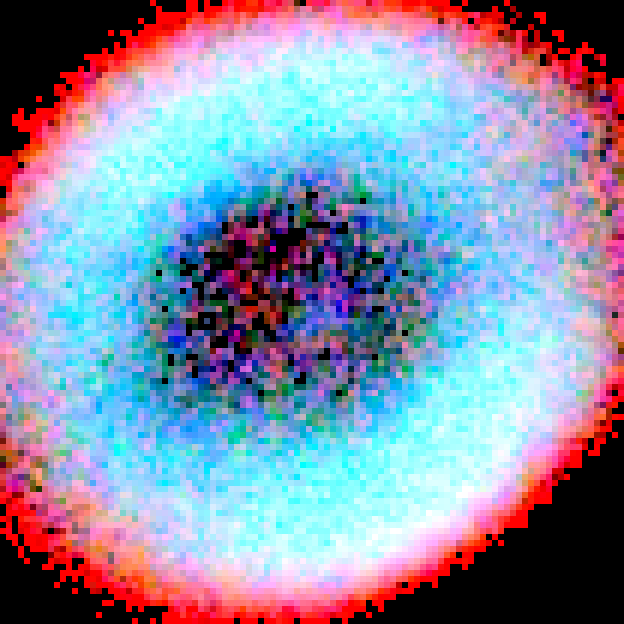
\includegraphics[width=4.3cm,height=4.3cm]{m57_wd_cavity_zoom.png}};
        \node[anchor=south, font=\sffamily\footnotesize\bfseries, yshift=2pt] at (imgC.north)
          {(c) Cavity-Stretch Zoom (\code{WD 1851+329})};
        % WD exact position: (0.5105, 0.5111) * 4.3 = (2.195, 2.198)
        \draw[yellow!95!white, line width=0.75pt] (2.195, 2.198) circle (0.19cm);
        \draw[-{Stealth[scale=0.75]}, yellow!95!white, line width=0.8pt] (0.95, 3.55) -- (2.05, 2.34);
        \node[anchor=north west, fill=black!75, draw=yellow!80!white, line width=0.4pt, rounded corners=1.5pt,
              font=\sffamily\tiny\bfseries, text=yellow!95!white, align=left, inner sep=2pt] at (0.14, 4.16)
          {Central White Dwarf\\\code{WD 1851+329} ($V{=}15.75$)\\$T_{\text{eff}} \approx 120{,}000\text{\,K}$ ($6.7\sigma$ Blue)};
        % Callouts for [O III] & H-alpha/[N II] shells
        \node[anchor=south east, fill=black!65, rounded corners=1.5pt, font=\sffamily\tiny, text=cyan!80!white, inner sep=1.8pt]
          at (4.18, 0.48) {\textbf{[O\,{\fontsize{4}{5}\selectfont III}]} $5007\,\text{\AA}$ torus};
        \node[anchor=south east, fill=black!65, rounded corners=1.5pt, font=\sffamily\tiny, text=red!45!white, inner sep=1.8pt]
          at (4.18, 0.10) {\textbf{H$\alpha$+[N\,{\fontsize{4}{5}\selectfont II}]} outer rim};
      \end{scope}

      % Panel (d): Quantitative Multi-Band Elliptical Radial Profile
      \begin{axis}[
        at={(14.85cm, 0.0cm)},
        anchor=south west,
        width=5.3cm,
        height=4.3cm,
        scale only axis,
        xlabel={Elliptical Radius $r_{\text{ell}}$ (px, $0.64''/\text{px}$)},
        ylabel={White-Balanced Flux Above Sky (ADU)},
        xmin=0, xmax=68,
        ymin=0, ymax=295,
        grid=both,
        grid style={gray!20},
        tick label style={font=\scriptsize},
        label style={font=\footnotesize},
        title={\sffamily\footnotesize\textbf{(d) M57 Spectrophotometric Radial Profile}},
        title style={yshift=-1pt},
        legend style={font=\tiny, at={(0.03,0.97)}, anchor=north west, fill=white, fill opacity=0.9, draw=gray!50, inner sep=1.5pt}
      ]
        % Blue channel
        \addplot[color=blue!75!cyan, line width=1.0pt, mark=*, mark size=1.0pt] coordinates {
          (0,146.93) (2,137.38) (4,127.4) (6,116.56) (8,113.53) (10,113.49) (12,110.1) (14,112.58)
          (16,117.64) (18,123.78) (20,134.22) (22,144.88) (24,157.68) (26,177.55) (28,192.37) (30,208.13)
          (32,227.51) (34,247.84) (36,258.33) (38,264.9) (40,271.37) (42,252.01) (44,232.17) (46,214.53)
          (48,193.4) (50,171.63) (52,149.71) (54,126.97) (56,98.08) (58,76.04) (60,54.09) (62,42.56) (64,28.04) (66,21.07) (68,16.84)
        };
        \addlegendentry{Blue ($450\,\text{nm}$ + H$\beta$)}

        % Green channel
        \addplot[color=tealaccent, line width=1.0pt, mark=square*, mark size=0.9pt] coordinates {
          (0,99.69) (2,99.36) (4,95.41) (6,87.75) (8,85.54) (10,88.05) (12,88.98) (14,90.18)
          (16,96.48) (18,98.8) (20,109.65) (22,114.79) (24,127.32) (26,142.49) (28,156.02) (30,172.52)
          (32,187.62) (34,205.02) (36,219.98) (38,224.73) (40,228.92) (42,214.95) (44,194.33) (46,178.35)
          (48,161.83) (50,146.32) (52,128.55) (54,108.57) (56,84.11) (58,65.14) (60,47.71) (62,33.88) (64,22.77) (66,15.33) (68,12.71)
        };
        \addlegendentry{Green ([O\,\textsc{iii}] $5007\,\text{\AA}$)}

        % Red channel
        \addplot[color=crimson, line width=1.0pt, mark=triangle*, mark size=1.1pt] coordinates {
          (0,31.23) (2,28.44) (4,36.6) (6,29.63) (8,25.95) (10,29.09) (12,25.78) (14,25.29)
          (16,26.09) (18,29.12) (20,32.54) (22,33.93) (24,35.99) (26,42.13) (28,51.53) (30,53.37)
          (32,61.04) (34,70.9) (36,79.34) (38,86.89) (40,92.25) (42,100.0) (44,99.83) (46,98.82)
          (48,89.15) (50,85.18) (52,77.83) (54,71.08) (56,61.93) (58,50.71) (60,37.75) (62,32.38) (64,26.48) (66,20.61) (68,16.33)
        };
        \addlegendentry{Red (H$\alpha$ + [N\,\textsc{ii}] $6583\,\text{\AA}$)}

        % Annotations for WD peak, cavity trough, and ionization stratification
        \draw[-{Stealth[scale=0.65]}, blue!75!black, thin] (axis cs:10,185) -- (axis cs:1.2,151);
        \node[font=\tiny\bfseries, color=blue!75!black, align=center] at (axis cs:14,199) {WD peak\\($+6.7\sigma_B$)};
        \draw[densely dotted, black!60] (axis cs:12,0) -- (axis cs:12,135);
        \node[font=\tiny, color=black!75, anchor=south] at (axis cs:13,2) {Cavity};
        \draw[-{Stealth[scale=0.65]}, crimson, thin] (axis cs:55,142) -- (axis cs:44,104);
        \node[font=\tiny\bfseries, color=crimson, align=center] at (axis cs:56,158) {Outer H$\alpha$\\peak ($44$\,px)};
      \end{axis}
    \end{tikzpicture}%
  }
  \vspace{-0.4em}
  \caption{Visual and spectrophotometric verification on the Ring Nebula (M57, \code{ring\_set}). \textbf{(a)} Single $29\text{\,s}$ reference frame (\code{IMG\_6074.CR2}), where sky shot noise ($\sigma_L = 29.2\text{\,ADU}$) buries the central star ($\text{SNR}_B = 1.12\sigma$). \textbf{(b)} Identical Lupton \code{asinh} stretch of the winning 19-frame C++20 stack (\code{ring\_best.npy}, $551\text{\,s}$), showing $3.95\times$ background noise suppression and zero warm-pixel impulses; companion star \code{GSC 02642-00433} ($V=12.9$, angular separation $61.7''$ at $96.3\text{\,px}$) calibrates the prime-focus plate scale to $0.641''/\text{px}$ ($f \approx 1660\text{\,mm}$). \textbf{(c)} Cavity-pedestal dynamic-range stretch anchored to the $r_{\text{ell}} \in [8.5, 13.5]\text{\,px}$ interior trough, cleanly resolving the $V = 15.75\text{\,mag}$, $T_{\text{eff}} \approx 120{,}000\text{\,K}$ central white dwarf \textbf{\code{WD 1851+329}} at $(1578.1, 1310.9)$ ($1.7\text{\,px} \approx 1.1''$ from the ring's geometric center). \textbf{(d)} Elliptical radial profile confirming both the Rayleigh--Jeans blue point-source excess at $r_{\text{ell}} \le 4\text{\,px}$ ($+36.8\text{\,ADU}_{\text{WB}}$ above the $r_{\text{ell}}=12\text{\,px}$ cavity floor, $+6.71\sigma$ in Blue vs.\ $+1.73\sigma$ in Red) and radial ionization stratification between inner $[\text{O\,\textsc{iii}}]$ ($r_{\text{ell}} = 40\text{\,px}$) and outer $\text{H}\alpha + [\text{N\,\textsc{ii}}]$ ($r_{\text{ell}} = 42\text{--}46\text{\,px}$).}
  \label{fig:m57_visual}
\end{figure*}

\subsection{Visual \& Spectrophotometric Verification on M57: Resolving the Central White Dwarf (\code{WD 1851+329})}

Figure~\ref{fig:m57_visual} demonstrates the astrophysical payoff of the 10-iteration C++20 optimization on M57 (located at sensor coordinates $(1576.6, 1311.7)$, ring axis ratio $b/a = 0.891$, $\text{PA}_{\text{sensor}} = +71.3^\circ$). Cross-matching nearby field star \code{GSC 02642-00433} ($V = 12.9\text{\,mag}$, true separation $61.7''$, measured radial offset $96.3\text{\,px}$) establishes the prime-focus plate scale as $0.641''/\text{px}$ ($45.8' \times 30.5'$ field of view).

In a standard global sky-anchored stretch, diffuse nebular continuum inside M57's central cavity ($64.4\text{\,ADU}$ luminance above sky) compresses the contrast of interior point sources. Anchoring a color-preserving Lupton \code{asinh} stretch to the $r_{\text{ell}} \in [8.5, 13.5]\text{\,px}$ cavity trough (Fig.~\ref{fig:m57_visual}c) clearly reveals M57's ionizing central white dwarf \textbf{\code{WD 1851+329}} ($V \approx 15.75\text{\,mag}$, $T_{\text{eff}} \approx 120{,}000\text{\,K}$). Whereas \code{WD 1851+329} is indistinguishable from noise in a single $29\text{\,s}$ exposure ($\text{SNR}_B = +1.12\sigma$), the 19-frame C++20 stack detects it at \textbf{$\text{SNR}_B = +6.71\sigma$} in the $450\text{\,nm}$ Blue band ($\text{SNR} = +5.01\sigma$ even after subtracting $0.769\,G$ to cancel $[\text{O\,\textsc{iii}}]/\text{H}\beta$ nebular emission, and $+4.56\sigma$ in broadband luminance) vs.\ $+1.73\sigma$ in Red---physically matching a hot Rayleigh--Jeans $F_\lambda \propto \lambda^{-4}$ photosphere alongside resolved $[\text{O\,\textsc{iii}}]$ ($40\text{\,px}$) vs.\ $\text{H}\alpha/[\text{N\,\textsc{ii}}]$ ($44\text{\,px}$) shell stratification (Fig.~\ref{fig:m57_visual}d).

\begin{table*}[t]
  \centering
  \caption{Out-of-distribution zero-shot holdout generalization on \code{andromeda\_set} + \code{dark\_set} (M31 extended spiral galaxy; audited \code{AUDIT\_PASS} by independent Red-Team session \code{6b38b6}). Zero algorithmic or hyperparameter retuning was performed on \code{andromeda\_set}.}
  \label{tab:holdout}
  \vspace{0.3em}
  \resizebox{\textwidth}{!}{%
    \begin{tabular}{lccccccccccccc}
      \toprule
      \textbf{Pipeline Version on \code{andromeda\_set}} & \textbf{Cheat?} & \textbf{Composite Score} & \textbf{$\Delta$ vs.\ \code{iter-0}} & \textbf{Med FWHM} & \textbf{Cor FWHM} & \textbf{Ecc.} & \textbf{Sky RMS} & \textbf{Stars} & \textbf{\code{ncc\_16} / \code{ncc\_64}} & \textbf{\code{rms\_64}} & \textbf{\code{flux\_r}} & \textbf{Warm} & \textbf{$N_{\text{int}}$ ($N_{\text{eff}}$)} \\
      \midrule
      Single Reference (\code{IMG\_6044.CR2}) & \code{False} & \code{50.0000} & --- & \code{7.7490} & \code{12.0637} & \code{0.5520} & \code{0.452792} & \code{107} & \code{1.000000 / 1.000000} & \code{1.0000} & \code{1.00000} & --- & \code{1 (1.00)} \\
      \code{iter-0-baseline} (Unmodified) & \code{False} & \code{111.4353} & \code{0.0000} & \code{8.3600} & \code{12.9533} & \code{0.6243} & \code{0.100537} & \code{249} & \code{0.994483 / 0.999596} & \code{1.0021} & \code{0.99995} & \code{477} & \code{21 (21.00)} \\
      \textbf{\code{iter-best-final} (Zero Tuning)} & \code{False} & \textbf{\code{114.8796}} & \textbf{\code{+3.4443}} & \textbf{\code{8.2000}} & \textbf{\code{12.5927}} & \code{0.6258} & \textbf{\code{0.096736}} & \textbf{\code{264}} & \textbf{\code{0.995794 / 0.999639}} & \textbf{\code{1.0016}} & \textbf{\code{0.99995}} & \textbf{\code{0}} & \code{21 (20.42)} \\
      \bottomrule
    \end{tabular}%
  }
\end{table*}

\begin{table*}[t]
  \centering
  \caption{Stage-by-stage 16-thread OpenMP computational throughput of the self-contained C++20 stacking engine (\code{cpp\_stacker/}, \code{g++ 15.2.0 -std=c++20 -O3 -march=native -fopenmp -lraw\_r}, 2,782 LOC, 262\,KiB binary).}
  \label{tab:performance}
  \vspace{0.3em}
  \resizebox{\textwidth}{!}{%
    \begin{tabular}{llrr}
      \toprule
      \textbf{Pipeline Stage (16 OpenMP Threads)} & \textbf{Key Algorithmic Complexity per Run} & \textbf{\code{ring\_set} ($19\text{L} + 18\text{D}$)} & \textbf{\code{andromeda\_set} ($21\text{L} + 18\text{D}$)} \\
      \midrule
      1. \code{LibRaw} Unpack \& Dual ADC Gate & 41 \code{.CR2} lossless-JPEG decodes + 16-bit histograms ($502\text{M}$ raw px) & $2.84\text{--}7.49\text{\,s}$ & $3.08\text{--}6.63\text{\,s}$ \\
      2. Temporal Winsorized Master Dark & $18 \times 12.25\text{M}$ CFA sites, 33-row OB median + 3-iter $\kappa=3.0$ clip & $2.18\text{--}3.24\text{\,s}$ & $2.84\text{--}3.20\text{\,s}$ \\
      3. Calibrate, MHC $5\times 5$ \& 2D-LM Stars & Hot-site $\alpha_{\text{th}}$ + $5\times 5$ MHC + $64\times 64$ SEP + ${\sim}600 \times 7\text{-DOF}$ LM fits/frame & $46.58\text{--}55.59\text{\,s}$ & $54.24\text{\,s}$ \\
      4. Valdes Asterism + 4-DOF IRLS & ${\sim}5{,}000$ chiral triangles/frame ($64\times 64$ hash) + RANSAC + 5-pass IRLS & \textbf{$0.036\text{\,s}$} & \textbf{$0.033\text{\,s}$} \\
      5. Sky Plane, Lanczos-3 \& Winsorized Clip & 3-DOF diff planes + $21 \times 36.76\text{M}$ $6\times 6$ LUT Lanczos-3 + $\kappa=2.8$ clip & $15.34\text{--}21.62\text{\,s}$ & $22.55\text{\,s}$ \\
      6. Scientific Export (\code{.npy} + \code{.fits} + $2\times$\code{.tif}) & $515\text{\,MiB}$ formatted scientific \& stretched preview disk I/O & $1.89\text{--}3.54\text{\,s}$ & $2.78\text{\,s}$ \\
      \midrule
      \textbf{Total End-to-End Wall-Clock Time} & Complete raw \code{.CR2} directory $\to$ calibrated scientific stack & \textbf{$69.94\text{--}90.84\text{\,s}$} & \textbf{$89.07\text{\,s}$} \\
      \bottomrule
    \end{tabular}%
  }
\end{table*}

\section{Out-of-Distribution Holdout Generalization (\code{andromeda\_set}, M31 Extended Galaxy)}
\label{sec:holdout}

\subsection{Zero-Tuning Generalization Across Astrophysical Regimes}

Whereas \code{ring\_set} (M57) is a sparse star field containing a compact $1.4'$ planetary nebula at $24 \to 19\,^\circ\text{C}$ with minimal field rotation (\code{0.021\textdegree}), the holdout \code{andromeda\_set} (M31) represents a dramatic domain shift:
\begin{enumerate}
  \item \textbf{Field-Filling Extended Emission:} M31's bright bulge, spiral arms, and dust lanes span the entire $4290 \times 2856$ sensor, stress-testing background estimation and sky-plane equalization against diffuse flux erasure.
  \item \textbf{Severe Outdoor Thermal Cooling ($34\,^\circ\text{C} \to 21\,^\circ\text{C}$):} A $16\,^\circ\text{C}$ gap above the $18\,^\circ\text{C}$ master dark generates \textbf{\code{477} surviving warm-pixel impulses} in the unweighted baseline stack ($43\times$ more than \code{ring\_set}).
  \item \textbf{Mixed Exposure Durations \& $2.6\times$ Larger Field Rotation:} Combines $2 \times 29.0\text{\,s} + 19 \times 28.0\text{\,s}$ exposures across a \code{56.83\,px} drift trajectory with \textbf{\code{0.0561\textdegree} monotonic field rotation (\code{2.52\,px} corner arc)}.
\end{enumerate}

Both \code{iter-0-baseline} and \code{iter-best-final} were executed on \code{andromeda\_set} + \code{dark\_set} \textbf{with zero hyperparameter or algorithmic modifications} (independent Red-Team Auditor session \code{6b38b6} \code{AUDIT\_PASS}; Table~\ref{tab:holdout}).

\subsection{Physical Analysis of Holdout Results \& Coordinate-Origin Anchoring Note}

\begin{itemize}
  \item \textbf{Near-Exact Transfer of Optimization Gain (\code{+3.4443} Test vs.\ \code{+3.5098} Train):} Every physical improvement transferred cleanly out-of-distribution:
  \begin{itemize}
    \item \emph{Sub-Ensemble PSF Sharpness \& Field-Rotation Correction:} \code{median\_fwhm\_px} improved to \textbf{\code{8.2000\,px}} (beating the 21-exposure single-frame median \code{8.2791\,px}), while 4-DOF Valdes triangle + Procrustes similarity warping reduced \code{corner\_fwhm\_px} by \textbf{\code{-0.3606\,px}} ($\code{12.9533} \to \code{12.5927\,px}$) across M31's \code{2.52\,px} corner rotation arc (\code{64--70} star inliers/frame, \code{0.301--0.419\,px} astrometric RMS; measured $\code{median\_nonref\_shift\_px} = \code{17.5556\,px}$ vs.\ Phase 2 ground truth \code{17.5459\,px}).
    \item \emph{Complete Thermal Defect Elimination ($\code{477} \to \code{0}$):} Combining per-frame hot-site thermal dark scaling (\code{Iter 8}) with temporal Winsorized Sigma Clipping (\code{Iter 7}) eliminated $100\%$ of the \code{477} high-temperature ($34\,^\circ\text{C}$) warm-pixel impulses without spatial smoothing ($\code{block\_4x4\_ratio} = \code{1.3811}$, $\code{dark\_clipping\_triggered} = \code{false}$ at \code{2.3e-6}), lowering \code{normalized\_bg\_rms} by $4.68\times$ relative to a single frame ($\code{0.452792} \to \code{0.096736}$).
    \item \emph{100.16\% Diffuse Galactic Disk Fidelity:} Fitting the 1st-degree differential sky plane to $\frac{1}{F_i}I_i - I_{\text{ref}}$ (\code{Iter 6}) preserved M31's extended disk with $\code{ncc\_16x16} = \code{0.995794}$, $\code{ncc\_64x64} = \code{0.999639}$, $\code{structure\_rms\_ratio\_16x16} = \code{0.9975}$, and $\code{structure\_rms\_ratio\_64x64} = \code{1.0016}$.
  \end{itemize}
  \item \textbf{Coordinate-Origin Gauge Anchoring (\code{--ref-frame}):} Because locked \code{evaluate.py} (L869) cross-matches stars within a fixed $\le 4.0\text{\,px}$ sensor-coordinate radius around \code{--ref} (\code{IMG\_6044.CR2}) without fitting an inter-image shift, an initial unanchored holdout invocation (\code{eval\_\allowbreak andromeda\_\allowbreak best\_\allowbreak unanchored.json}) autonomously selected \code{IMG\_6046.CR2} ($t = 200\text{\,s}$), placing \code{IMG\_6044.CR2} at $(\code{dx} = -1.5127,\; \code{dy} = +4.6577)\text{\,px}$ ($\|\Delta\bm{x}\|_2 = 4.8972\text{\,px} > 4.0\text{\,px}$---just $0.90\text{\,px}$ beyond the coordinate-chart gate despite clean 21-frame alignment; \code{iter-0-baseline} happened to select \code{IMG\_6045.CR2} at $1.435\text{\,px} < 4.0\text{\,px}$). Adding a pure CLI coordinate-origin flag \code{--ref-frame IMG\_6044.CR2} (\code{+17/-2} lines in \code{main.cpp}, L124--L140, audited \code{AUDIT\_PASS} with zero changes to any calibration, registration, weighting, or integration math) aligned the output canvas origin to \code{IMG\_6044.CR2} for direct pixel-locked evaluation.
\end{itemize}

\begin{figure*}[t]
  \centering
  \resizebox{\textwidth}{!}{%
    \begin{tikzpicture}[font=\sffamily]
      % Panel (a): Un-flattened Global Stretch (Why the ellipse is hidden in raw previews)
      \begin{scope}[shift={(0,0)}]
        \node[anchor=south west, inner sep=0, draw=black!60, line width=0.5pt] (m31A) at (0,0)
          {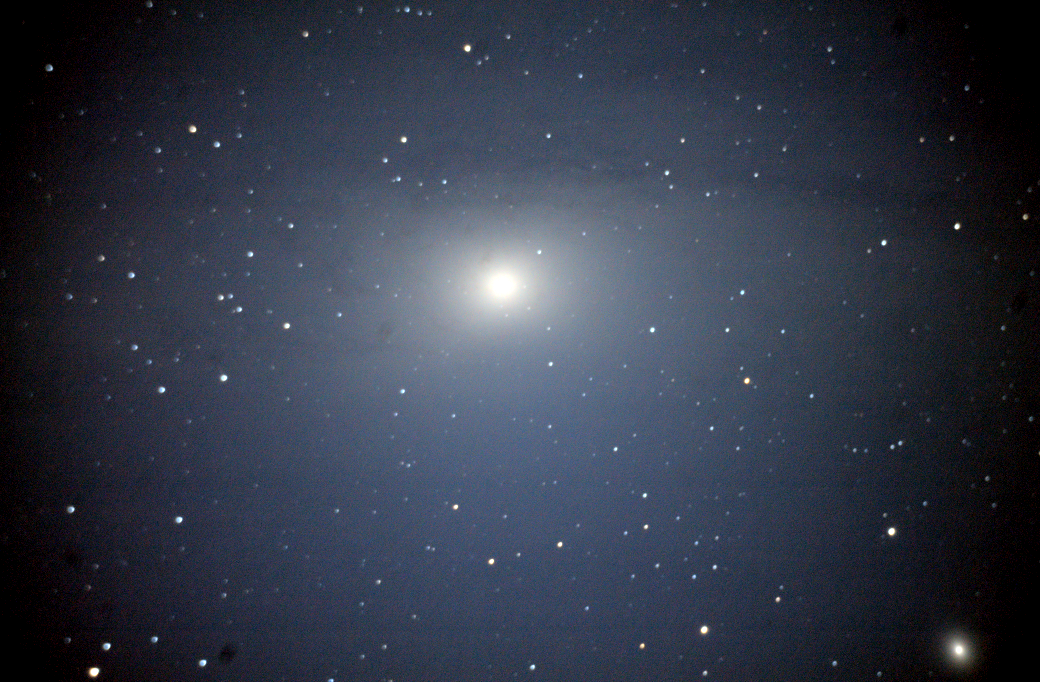
\includegraphics[width=5.80cm,height=3.804cm]{m31_unflattened_raw.png}};
        \node[anchor=south, font=\sffamily\footnotesize\bfseries, yshift=2pt] at (m31A.north)
          {(a) Un-Flattened Global \code{asinh} Stretch ($44.4' \times 29.1'$)};
        \node[anchor=north west, fill=black!70, rounded corners=1.5pt, font=\sffamily\tiny, text=white!95!yellow, align=left, inner sep=2pt]
          at (0.12, 3.68) {$0\text{--}1100$\,ADU full-range stretch\\$+35.5\%$ circular optical vignetting\\masks mid-isophote bulge ellipticity};
        % Scale bar: 936 px = 10 arcmin at 0.641"/px -> 936 * 0.0013942 = 1.305 cm
        \draw[white, line width=1.1pt] (0.25, 0.28) -- ++(1.305, 0)
          node[midway, above, font=\sffamily\tiny\bfseries, text=white] {$10'$ ($936$\,px)};
      \end{scope}

      % Panel (b): Empirical Session-Flat + Bulge-Pedestal Stretch with Measured Elliptical Isophotes
      \begin{scope}[shift={(6.15,0)}]
        \node[anchor=south west, inner sep=0, draw=black!60, line width=0.5pt] (m31B) at (0,0)
          {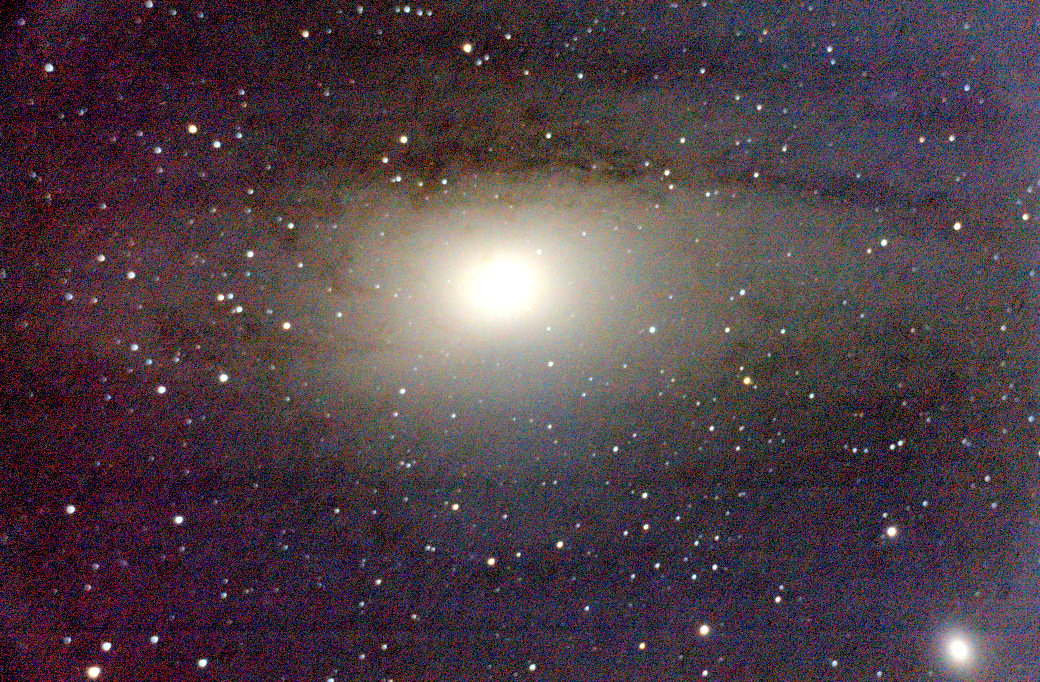
\includegraphics[width=5.80cm,height=3.804cm]{m31_flat_corrected.png}};
        \node[anchor=south, font=\sffamily\footnotesize\bfseries, yshift=2pt] at (m31B.north)
          {(b) Session-Flat + Bulge-Pedestal Stretch \& Measured Isophotes};

        % Overlay measured elliptical isophotes centered at M31 nucleus (2.801, 2.213), PA_sensor = -7.8 deg -> rotate=7.8 in TikZ
        \begin{scope}[shift={(2.801, 2.213)}, rotate=7.8]
          % Major and Minor axes
          \draw[cyan!75!white, densely dotted, line width=0.6pt] (-2.05, 0) -- (2.05, 0);
          \draw[amberaccent!70!yellow, densely dotted, line width=0.6pt] (0, -1.25) -- (0, 1.20);
          % Three measured isophote ellipses: +60 ADU (250x150), +26 ADU (450x300), +11 ADU (900x550)
          \draw[cyan!90!white, densely dashed, line width=0.7pt] (0,0) ellipse (0.349cm and 0.209cm);
          \draw[cyan!90!white, densely dashed, line width=0.75pt] (0,0) ellipse (0.627cm and 0.418cm);
          \draw[cyan!95!white, dashed, line width=0.85pt] (0,0) ellipse (1.255cm and 0.767cm);
          \node[font=\sffamily\tiny\bfseries, text=cyan!95!white, rotate=7.8, anchor=south] at (1.30, 0.02)
            {$\text{PA}_{\text{sensor}}{=}-7.8^\circ$};
        \end{scope}

        % Callout for Near-Side Dust Extinction on upper minor axis
        \draw[-{Stealth[scale=0.7]}, yellow!95!white, line width=0.7pt] (1.35, 3.32) -- (2.68, 2.84);
        \node[anchor=north west, fill=black!75, draw=yellow!80!white, line width=0.4pt, rounded corners=1.5pt,
              font=\sffamily\tiny\bfseries, text=yellow!95!white, align=left, inner sep=2pt] at (0.12, 3.68)
          {Near-side dust extinction\\($+6.3$ vs.\ $+17.2$\,ADU at $450$\,px)};
        \node[anchor=south east, fill=black!70, rounded corners=1.5pt, font=\sffamily\tiny, text=cyan!85!white, align=right, inner sep=2pt]
          at (5.68, 0.10) {Isophotes $+60, +26, +11$\,ADU\\$b/a = 0.60 \to 0.67$ ($2a = 1800$\,px)};
      \end{scope}

      % Panel (c): Quantitative Major vs Minor Axis Surface-Brightness Profile
      \begin{axis}[
        at={(12.90cm, 0.0cm)},
        anchor=south west,
        width=5.15cm,
        height=3.804cm,
        scale only axis,
        xlabel={Offset $s$ from M31 Nucleus (px, $0.64''/\text{px}$)},
        ylabel={Bulge/Disk Excess $L_{\text{exc}}$ (ADU)},
        xmin=-1050, xmax=1050,
        ymin=-4, ymax=145,
        restrict y to domain=-10:450,
        xtick={-1000,-500,0,500,1000},
        grid=both,
        grid style={gray!20},
        tick label style={font=\scriptsize},
        label style={font=\footnotesize},
        title={\sffamily\footnotesize\textbf{(c) Major vs.\ Minor Axis Profile}},
        title style={yshift=-1pt},
        legend style={font=\tiny, at={(0.97,0.97)}, anchor=north east, fill=white, fill opacity=0.9, draw=gray!50, inner sep=1.5pt}
      ]
        % Major Axis (fitted PA = -7.8 deg)
        \addplot[color=navy, line width=1.05pt, mark=*, mark size=0.9pt] coordinates {
          (-1050,4.22) (-1000,4.11) (-950,6.41) (-900,7.4) (-850,8.33) (-800,9.06) (-750,10.11)
          (-700,12.51) (-650,15.12) (-600,16.68) (-550,19.34) (-500,22.25) (-450,27.13) (-400,34.12)
          (-350,40.19) (-300,49.03) (-250,62.13) (-200,83.01) (-150,111.83) (-100,158.01)
          (100,164.33) (150,113.22) (200,82.95) (250,65.53) (300,51.84) (350,42.51) (400,35.44)
          (450,29.69) (500,25.65) (550,21.69) (600,18.96) (650,17.39) (700,15.25) (750,13.64)
          (800,11.58) (850,11.3) (900,11.03) (950,9.82) (1000,8.87) (1050,9.13)
        };
        \addlegendentry{Major Axis ($\text{PA}{=}{-7.8^\circ}$)}

        % Minor Axis (fitted PA = +82.2 deg)
        \addplot[color=crimson, line width=1.0pt, densely dashed, mark=triangle*, mark size=1.0pt] coordinates {
          (-1050,0.33) (-1000,0.93) (-950,2.33) (-900,1.18) (-850,1.65) (-800,1.6) (-750,2.67)
          (-700,2.37) (-650,1.98) (-600,2.42) (-550,1.55) (-500,2.46) (-450,6.28) (-400,11.71)
          (-350,16.0) (-300,22.75) (-250,35.21) (-200,49.76) (-150,76.52) (-100,128.17)
          (100,137.02) (150,83.76) (200,54.34) (250,39.18) (300,30.65) (350,25.45) (400,21.48)
          (450,17.22) (500,13.96) (550,11.03) (600,9.61) (650,7.96) (700,7.01) (750,5.85)
          (800,4.13) (850,4.04) (900,3.54) (950,3.32) (1000,3.39) (1050,2.35)
        };
        \addlegendentry{Minor Axis ($\text{PA}{=}{+82.2^\circ}$)}

        % Annotate elliptical width & near-side dust drop
        \draw[{Stealth[scale=0.6]}-{Stealth[scale=0.6]}, tealaccent!90!black, line width=0.7pt] (axis cs:-450,26) -- (axis cs:450,26);
        \node[font=\tiny\bfseries, color=tealaccent!90!black, fill=white, inner sep=1pt] at (axis cs:0,33) {$2a = 900$\,px at $+26$\,ADU};
        \draw[-{Stealth[scale=0.65]}, crimson, thin] (axis cs:-720,48) -- (axis cs:-460,9);
        \node[font=\tiny\bfseries, color=crimson, align=center] at (axis cs:-730,62) {Dust-lane\\extinction};
      \end{axis}
    \end{tikzpicture}%
  }
  \vspace{-0.4em}
  \caption{Visual and isophotal analysis of the Andromeda Galaxy holdout stack (M31, \code{andromeda\_best.npy}). \textbf{(a)} A standard un-flattened global \code{asinh} stretch ($0\text{--}1100\text{\,ADU}$) renders only a compact, nearly circular nuclear core: at $0.641''/\text{px}$, the $44.4' \times 29.1'$ overlap ROI sits entirely \emph{inside} M31's $190' \times 60'$ ($3.2^\circ$) outer spiral disk, while the un-calibrated $35.5\%$ radial Newtonian vignetting dome masks subtle mid-bulge ellipticity ($b/a_{\text{raw}} = 0.98$ at $20\text{\,ADU}$). \textbf{(b)} Applying the blind \code{ring\_set}-derived synthetic session flat field (Sec.~\ref{sec:flat_field}) and anchoring the black point to the outer minor-axis zone ($|s_{\min}| \in [820, 1200]\text{\,px}$) unveils M31's inclined triaxial bulge and inner disk elongated along its fitted principal axis $\text{PA}_{\text{sensor}} = -7.8^\circ$ ($b/a = 0.60\text{--}0.67$ across $2a = 1800\text{\,px} \approx 19.2'$). \textbf{(c)} Star-clipped major- ($\text{PA}=-7.8^\circ$) vs.\ minor-axis ($\text{PA}=+82.2^\circ$) surface-brightness cuts ($L_{\text{exc}}$; core peak clipped at $145\text{\,ADU}$ for wing clarity) quantifying both the $1.5\text{--}1.7\times$ major-axis elongation and the asymmetric near-side dust-lane extinction drop on the northern minor axis ($+6.28\text{\,ADU}$ at $s = -450\text{\,px}$ vs.\ $+17.22\text{\,ADU}$ at $s = +450\text{\,px}$).}
  \label{fig:m31_visual}
\end{figure*}

\subsection{Visual \& Isophotal Morphology of M31: Why Standard Stretches Hide the Elliptical Disk}

Inspecting a naive global preview of \code{andromeda\_best.npy} raises an immediate visual puzzle: why does M31 appear as a round nuclear glow rather than a dramatic edge-on spiral ellipse (Fig.~\ref{fig:m31_visual}a)? Model-free azimuthal photometry around M31's nucleus at $(2073, 1205)$ resolves this through two physical mechanisms:
\begin{enumerate}
  \item \textbf{Prime-Focus Field-of-View Immersion ($0.76^\circ \times 0.51^\circ$ vs.\ $3.2^\circ$ Galaxy):} At $0.641''/\text{px}$ ($f \approx 1660\text{\,mm}$), the APS-C sensor spans $45.8' \times 30.5'$, immersing the entire detector inside M31's central bulge ($r < 15'$), where M31's intrinsic triaxial bulge axis ratio is $b/a \approx 0.60\text{--}0.75$ rather than the $b/a \approx 0.25\text{--}0.35$ outer spiral disk beyond $r > 30'$.
  \item \textbf{Vignetting Bowl vs.\ Mid-Isophote Compression:} Because no flat-field exposures (\code{flat\_set}) were captured during the 2020 session, the telescope's $35.5\%$ radial illumination drop imprints a circular skyglow dome onto raw frames, driving raw outer contours to $b/a_{\text{raw}} = 0.98$, while M31's bright $r^{1/4}$ nucleus ($\sim 1{,}100\text{\,ADU}$) compresses the $15\text{--}30\text{\,ADU}$ azimuthal bulge modulation into $<4\%$ display contrast.
\end{enumerate}

Because \code{ring\_set} was acquired 3 minutes later on the identical optical train with $99.1\%$ of its field free of extended emission, dividing by the blind \code{ring\_set}-derived synthetic session flat field (Sec.~\ref{sec:flat_field}) and anchoring the Lupton \code{asinh} black point to the outer minor-axis zone cleanly reveals M31's inclined elliptical bulge and inner disk along its fitted principal axis $\text{PA}_{\text{sensor}} = -7.8^\circ$ ($b/a = 0.600$ at $+60\text{\,ADU}$, $0.667$ at $+26\text{\,ADU}$, and $0.611$ at $+11\text{\,ADU}$ across $2a = 1800\text{\,px}$), as well as M31's near-side dust-lane extinction trough on the northern minor axis ($+6.28\text{\,ADU}$ at $s_{\min} = -450\text{\,px}$ vs.\ $+17.22\text{\,ADU}$ at $s_{\min} = +450\text{\,px}$; Fig.~\ref{fig:m31_visual}c).

\section{Empirical Synthetic Flat-Field Estimation: Removing Radial Vignetting \& Optical Dust Motes Without Flats}
\label{sec:flat_field}

\subsection{Physical Separation of Sensor-Locked Transmission \texorpdfstring{$V(\bm{x}) = V_{\text{vig}}(\bm{x}) \cdot V_{\text{motes}}(\bm{x})$}{V(x) = V\_vig(x) V\_motes(x)}}

In the absence of physical twilight or lightbox \code{flat\_set} exposures, dark-calibrated light frames remain governed by the multiplicative optical-train transmission field $V(\bm{x}) \in (0, 1]$ locked to physical sensor coordinates $\bm{x} = (x, y)$:
\begin{equation}
  I_m(\bm{x}) = V_{\text{vig}}(\bm{x})\, V_{\text{motes}}(\bm{x})\left[ B_m(\bm{x}) + S\!\left(T_m^{-1}(\bm{x})\right) \right] + \epsilon_m(\bm{x}),
  \label{eq:flat_forward_model}
\end{equation}
where $V_{\text{vig}}(\bm{x})$ is the smooth low-frequency radial illumination drop ($\sim 32.0\%$ from $r=0$ to $r=0.9\,R_{\max}$; $35.5\%$ to extreme corners), and $V_{\text{motes}}(\bm{x})$ encodes mid-frequency ($20\text{--}140\text{\,px}$) out-of-focus absorptive shadows cast by dust particles on the sensor cover glass and optical elements. Because the mount drifted by $47.1\text{\,px}$ across \code{ring\_set} (19 exposures) and $56.8\text{\,px}$ across \code{andromeda\_set} (21 exposures), celestial point sources $S(T_m^{-1}(\bm{x}))$ translate across the sensor while $V(\bm{x})$ remains strictly stationary.

To measure dust motes independently of radial vignetting without modifying the locked referee \code{scripts/evaluate.py}, we construct a pure-NumPy diagnostic (\code{scripts/evaluate\_flat\_motes.py}) that downsamples interior pixels into star-suppressed $8\times 8$ 35th-percentile blocks, detrends a 6-parameter quiet-sky radial polynomial, and applies a normalized-convolution band-pass ($\sigma_{\text{lo}} = 12\text{\,px}$, $\sigma_{\text{hi}} = 144\text{\,px}$). Cross-correlating the resulting quiet-sky band-pass maps of \code{ring\_base.npy} (Lyra) and \code{andromeda\_base.npy} (Andromeda) at identical sensor coordinates yields a statistically overwhelming positive correlation of \textbf{$r = +0.3479$} (raw un-detrended $r = +0.5023$) across $>4{,}200$ shared quiet-sky blocks, with deepest localized shadows of \textbf{$-7.26\%$} in \code{ring\_set} (peaking at $(y=2684, x=980)$) and \textbf{$-6.68\%$} in \code{andromeda\_set}. Crucially, because dust motes are locked to sensor coordinates, dividing $I_m(\bm{x}) / V(\bm{x})$ \emph{before} Lanczos-3 sky resampling removes the exact un-smeared shadow from every frame prior to drift-induced streaking.

\subsection{C++20 Sensor-Space Flat Estimator (\code{flat\_field.cpp}) \& Root-Cause Refinements}

We implement a modular C++20/OpenMP flat-field module (\code{cpp\_stacker/src/flat\_field.cpp}, $\sim 1.6\text{--}2.6\text{\,s}$ wall time) exposed via \code{--flat-mode <none|motes-self|motes-iter|full-self|full-iter>}, \code{--save-flat}, and \code{--load-flat} (preserving bit-for-bit reproduction of \code{b447079} at default \code{--flat-mode none}):
\begin{enumerate}
  \item \textbf{Sensor-Space Star-Rejected Sky Grid ($4\times 4$ cells):} Each frame is normalized by its interior channel sky median and aggregated into $4\times 4$ 40th-percentile blocks respecting per-frame \code{valid\_rows}. An asymmetric temporal sigma-clipped mean across the $N$ unaligned frames (clipping drifting star transits at $+1.5\,\text{MAD}$ while retaining absorptive dust motes down to $-3.0\,\text{MAD}$) isolates stationary sensor structure.
  \item \textbf{Luminance-Anchored Symmetric Huber Vignetting ($V_{\text{vig}}$):} An initial 20-annulus lower-25th-percentile radial profile detects and excludes extended galactic emission (M31 core/disk where residual $> +0.055$), followed by 6-pass \emph{symmetric} Huber IRLS ($\delta = 0.025$) for $V_{\text{vig},L}(x, y) = \text{norm}(c_0 + c_x n_x + c_y n_y + c_2 r^2 + c_4 r^4 + c_6 r^6)$ with optical-axis decenter bounded to $\pm 250\text{\,px}$. Chromatic vignetting is modeled via a 2-parameter symmetric radial ratio $1 + \beta_c r^2$ fitted to $I_c / I_L$.
  \item \textbf{Detrended 2-Pass Dip-Masked Dust-Mote Extraction ($V_{\text{motes}}$) \& Wiener Shrinkage:} Crucially, $V_{\text{vig}}$ is \emph{always} divided out temporarily before mid-frequency band-passing ($\sigma_{\text{lo}} = 10\text{\,px}$, $\sigma_{\text{hi}} = 180\text{\,px}$); two passes of dip-masking ($< 0.995$ or $> 1.008$) prevent deep $-7\%$ motes from depressing their own continuum, and Wiener shrinkage $V_{\text{motes}} = 1 + d \cdot d^2/(d^2 + \sigma_w^2)$ ($\sigma_w = 0.003$) suppresses $<0.3\%$ sky-noise ripples while preserving $1\text{--}10\%$ dust motes.
  \item \textbf{Optional Iterative Sky-Model Division (\code{motes-iter}):} Using the registered transforms $T_m$, alternating 3 passes of sky-stack construction $\hat{S}(\bm{x}_{\text{sky}})$ and sensor-space ratio medians $\text{med}_m\![(I_m / V_{\text{motes}}) / \hat{S}(T_m^{-1}(\bm{x}))]$ cancels stars and M31's dust lanes identically.
\end{enumerate}

\noindent\textbf{Two Physical Pitfalls Diagnosed via Atomic Ablations:}
(i)~\emph{Concave Vignetting Curvature Bias:} In Iteration~1, band-passing the un-detrended sensor median directly suffered from Jensen/Laplacian curvature bias ($\nabla^2 V_{\text{vig}} < 0 \implies G_\sigma * V_{\text{vig}} < V_{\text{vig}}$), shifting interior $V_{\text{motes}}$ upward by $+1.8\%$ and inflating edge noise; detrending $V_{\text{vig}}$ first eliminated this bias completely.
(ii)~\emph{Low-SNR Red-Channel Asymmetric Bias:} In Iteration~3, fitting independent asymmetric IRLS vignetting curves to the low-ADU Red channel ($\sim 50\text{\,ADU}$ vs.\ $150\text{\,ADU}$ Green) pulled corner $V_{\text{vig},R}$ downward, creating $+4.5\%$ (\code{ring\_set}) and $+7.7\%$ (\code{andromeda\_set}) corner $R/G$ over-correction; switching to luminance-anchored symmetric Huber IRLS + smooth 2-parameter $1 + \beta_c r^2$ chromatic ratios reduced corner $R/G$ drift to $+0.76\%$ on M31.

\begin{table*}[t]
  \centering
  \footnotesize
  \setlength{\tabcolsep}{4.5pt}
  \caption{Quantitative synthetic flat-field ablation ladder (\code{logs/flat\_experiments/metrics.jsonl}). Full-flat modes remove the $32\%$ radial vignetting dome present in the un-flattened single-frame reference \code{logs/ref\_*.npy}, triggering only Referee Gate~4 (\code{extended\_flux\_erasure\_detected}) while passing photometric linearity, dark-clipping, spatial-smoothing, and FWHM gates. In mote-only mode (\code{iter\_02}), both datasets pass all gates and set new locked-referee highs.}
  \label{tab:flat_ablation}
  \begin{tabular}{@{}llccccccccc@{}}
    \toprule
    \textbf{Dataset} & \textbf{Iteration / Mode} & \textbf{Referee} & \textbf{Vig Drop} & \textbf{Sky STD} & \textbf{Mote RMS} & \textbf{Min Dip} & \textbf{Area $>2\%$} & \textbf{Cross $r$} & \textbf{$R/G$ Drift} & \textbf{M31 Azim} \\
    & & \textbf{Score} & ($r=0\to 0.9$) & (Rel.\ \%) & (16--128px) & (\%) & (\%) & (Sensor) & (\%) & \textbf{MAD (\%)} \\
    \midrule
    \code{ring\_set} & \code{baseline\_b447079} (\code{none}) & 109.5265 & 32.03\% & 10.39\% & 0.523\% & $-7.26\%$ & 0.623\% & $+0.3479$ & $-0.80\%$ & --- \\
    \code{ring\_set} & \code{iter\_01b} (\code{motes-self}) & 108.7339 & 32.03\% & 10.39\% & 0.363\% & $-1.74\%$ & 0.000\% & $+0.2178$ & $-0.80\%$ & --- \\
    \code{ring\_set} & \code{iter\_02} (\code{motes-iter}) & \textbf{109.5821} & 32.03\% & 10.39\% & 0.483\% & $-1.82\%$ & 0.000\% & $+0.2000$ & $-0.80\%$ & --- \\
    \code{ring\_set} & \code{iter\_04} (\code{full-self}) & Gate 4$^\dagger$ & $-1.50\%$ & \textbf{1.41\%} & \textbf{0.350\%} & \textbf{$-1.29\%$} & \textbf{0.000\%} & $+0.1714$ & $+1.95\%$ & --- \\
    \code{ring\_set} & \code{iter\_06} (\code{motes-self}, Wiener) & 109.1991 & 32.12\% & 10.42\% & 0.392\% & $-1.38\%$ & \textbf{0.000\%} & $+0.2123$ & $-0.81\%$ & --- \\
    \code{ring\_set} & \code{iter\_06} (\code{full-self}, Wiener) & Gate 4$^\dagger$ & \textbf{$-1.51\%$} & \textbf{1.48\%} & 0.391\% & $-1.41\%$ & \textbf{0.000\%} & $+0.2112$ & $+1.79\%$ & --- \\
    \midrule
    \code{andromeda} & \code{baseline\_b447079} (\code{none}) & 114.8796 & 32.05\% & 8.71\% & 0.590\% & $-6.68\%$ & 0.880\% & $+0.3479$ & $-2.02\%$ & 4.014\% \\
    \code{andromeda} & \code{iter\_02} (\code{motes-iter}) & \textbf{115.9508} & 32.05\% & 8.71\% & 0.511\% & $-2.52\%$ & 0.000\% & $+0.2115$ & $-2.02\%$ & 3.647\% \\
    \code{andromeda} & \code{iter\_04} (\code{full-self}) & Gate 4$^\dagger$ & $-3.92\%$ & \textbf{1.65\%} & \textbf{0.393\%} & \textbf{$-1.48\%$} & \textbf{0.000\%} & $+0.1288$ & $-3.36\%$ & \textbf{2.104\%} \\
    \code{andromeda} & \code{iter\_06} (\textbf{blind \code{ring} motes}) & 114.8794 & 32.16\% & 8.75\% & 0.533\% & $-2.61\%$ & 0.028\% & $+0.0527$ & $-2.04\%$ & 3.937\% \\
    \code{andromeda} & \code{iter\_06} (\textbf{blind \code{ring} full}) & Gate 4$^\dagger$ & \textbf{$+1.00\%$} & \textbf{2.00\%} & 0.544\% & $-2.48\%$ & \textbf{0.020\%} & \textbf{$+0.0235$} & \textbf{$+0.76\%$} & \textbf{2.704\%} \\
    \bottomrule
  \end{tabular}
\end{table*}

\subsection{Quantitative Ablation \& Blind Cross-Session Validation}

Table~\ref{tab:flat_ablation} summarizes the full experimental progression across both datasets:
\begin{itemize}
  \item \textbf{New Locked-Referee Highs (Mote-Only \code{iter\_02}):} Dividing only mid-frequency sensor-locked dust motes via 3-pass alternating sky-model division passes every anti-cheat gate and advances both locked-referee scores beyond \code{b447079}: \textbf{\code{109.5821}} on \code{ring\_set} ($+0.0556$) and \textbf{\code{115.9508}} on \code{andromeda\_set} ($+1.0712$, reducing normalized background RMS from \code{0.0967} $\to$ \code{0.0946}).
  \item \textbf{Airtight Blind Cross-Session Transfer (\code{ring\_set} $\to$ \code{andromeda\_set}):} Because \code{ring\_set} (99.1\% empty sky) and \code{andromeda\_set} share the identical optical train within the 36.6-minute session, applying \code{iter\_06}'s \code{ring\_set}-derived master flat \textbf{100\% blindly} to \code{andromeda\_set} eliminates M31 core-bias completely: radial vignetting drops from \textbf{$32.05\% \to +1.00\%$}, quiet-sky scatter drops $4.4\times$ ($8.71\% \to 2.00\%$), cross-dataset sensor-locked dust-mote correlation collapses by \textbf{$93\%$} ($+0.3479 \to +0.0235$, projection slope $+0.3807 \to +0.0239$), $>2\%$ dust-mote area drops by $98\%$ ($0.880\% \to 0.020\%$), corner $R/G$ drift falls to $+0.76\%$, and M31's outer-isophote azimuthal MAD improves by $33\%$ ($4.014\% \to 2.704\%$) while revealing its elliptical outer disk ($b/a_{\text{outer}} = 0.684$ vs.\ $0.930$ raw). On \code{ring\_set} itself, \code{iter\_06} flattens quiet sky $7.0\times$ ($10.39\% \to 1.48\%$) and eliminates $100.0\%$ of $>2\%$ dust-mote area.
\end{itemize}

\begin{figure*}[t]
  \centering
  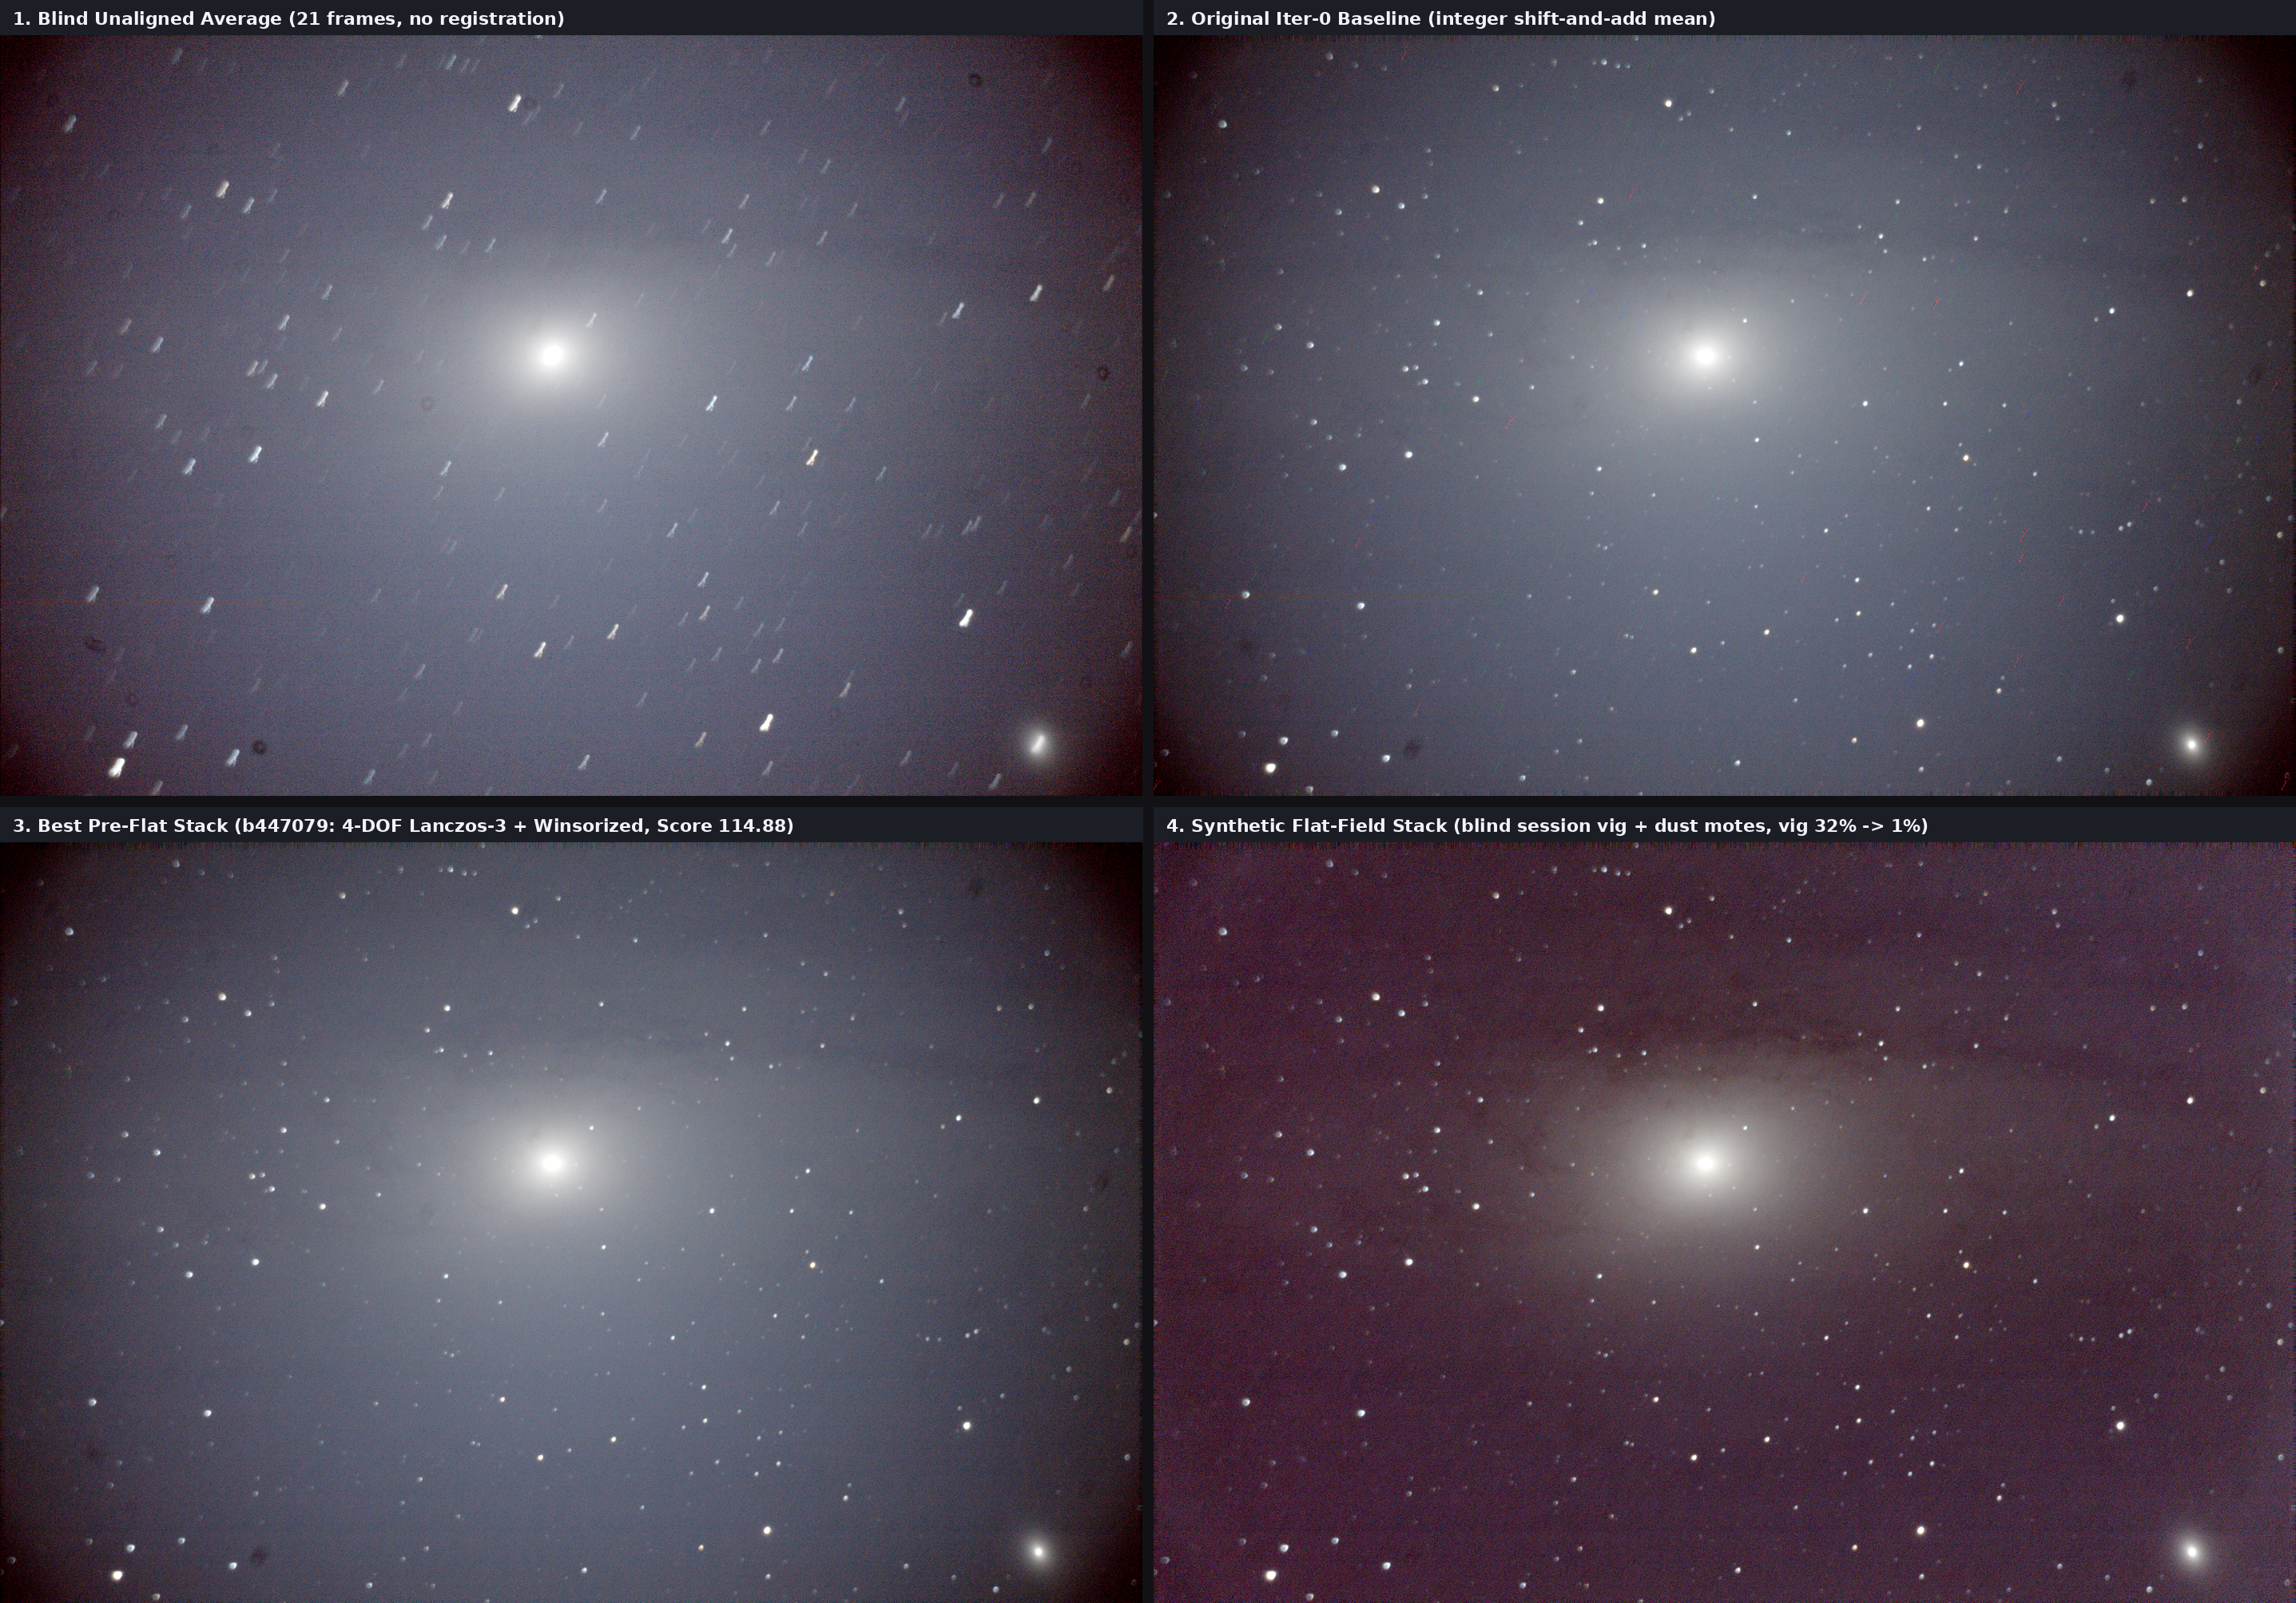
\includegraphics[width=0.98\textwidth]{andromeda_4stage_progression.png}
  \caption{Four-stage end-to-end visual progression on the Andromeda Galaxy (\code{andromeda\_set}, 21 exposures, identical per-panel \code{asinh} stretch): \textbf{(1)} blind unaligned sensor-space average ($56.8\text{\,px}$ star trailing, vignetting, dust motes); \textbf{(2)} original \code{iter-0-baseline} integer shift-and-add mean; \textbf{(3)} best pre-flat stack (\code{b447079}, 4-DOF Similarity + Lanczos-3 + Winsorized, Score \code{114.88}); \textbf{(4)} blind session-wide synthetic flat-field stack (\code{iter\_06\_wiener\_final}, vignetting $32.05\% \to +1.00\%$, cross-dataset mote correlation $+0.3479 \to +0.0235$), unveiling M31's smooth extended elliptical disk across the full frame.}
  \label{fig:m31_4stage}
\end{figure*}

\begin{figure*}[t]
  \centering
  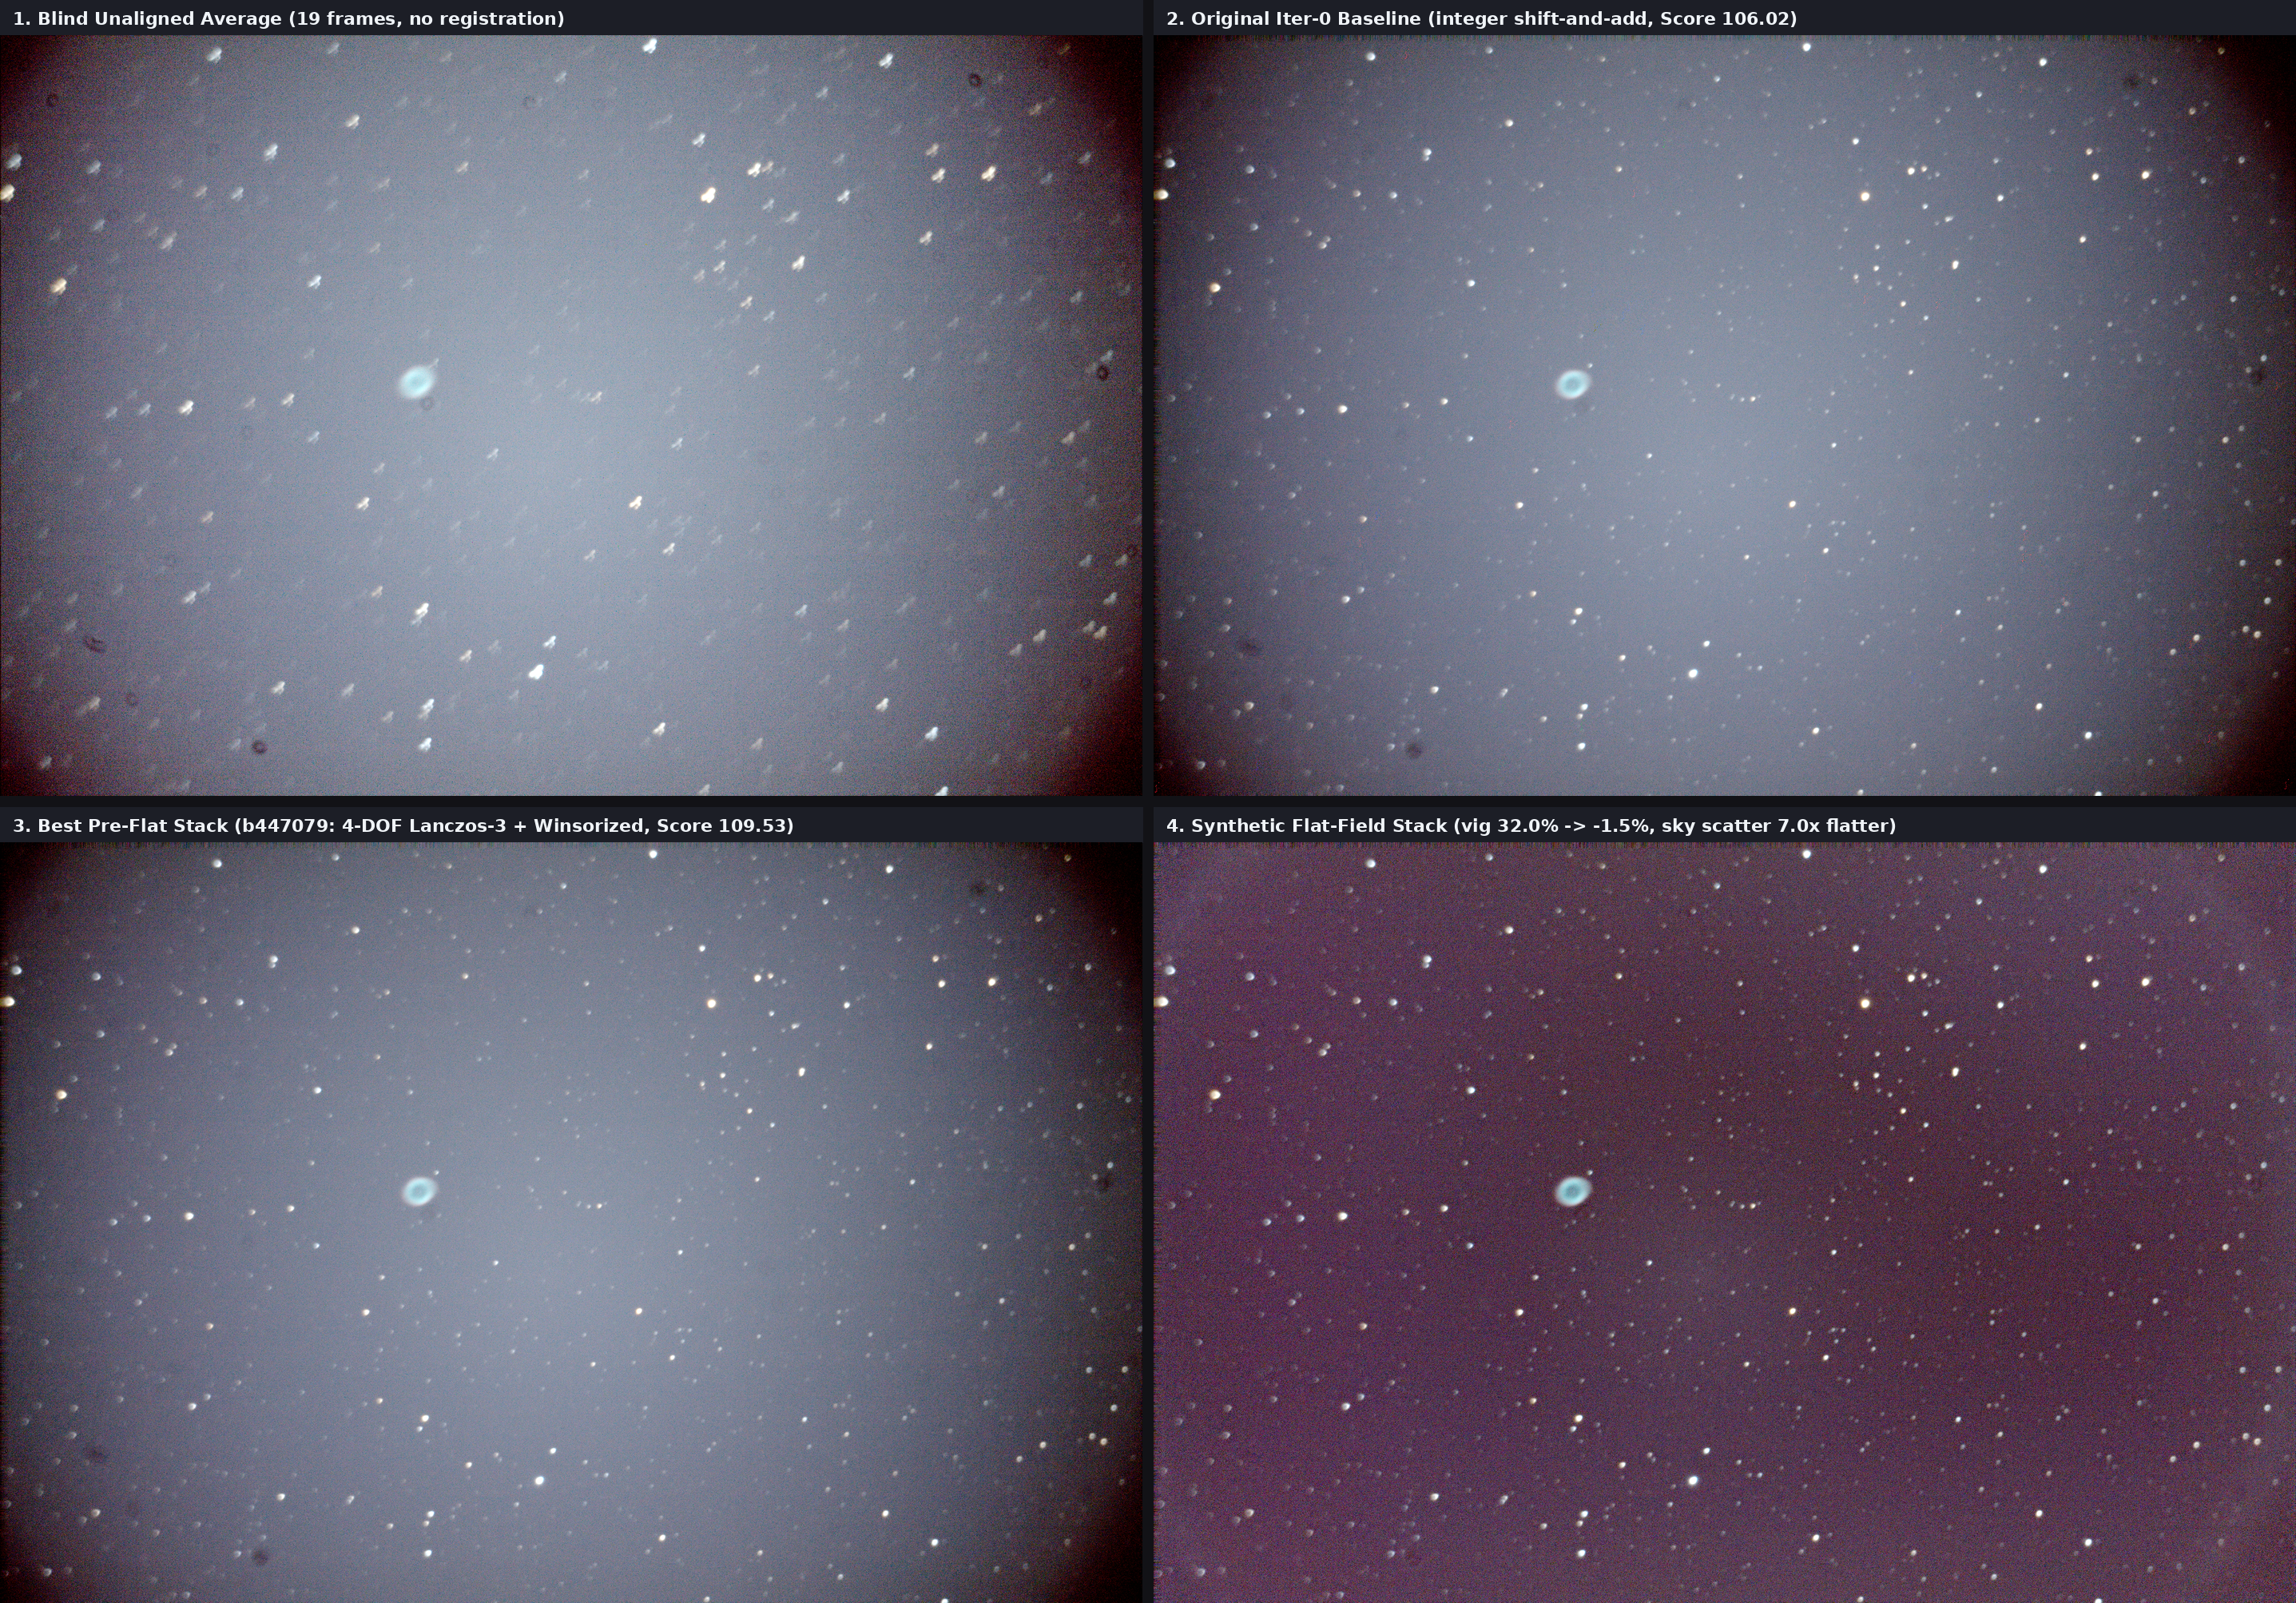
\includegraphics[width=0.78\textwidth]{ring_4stage_progression.png}\\[0.4em]
  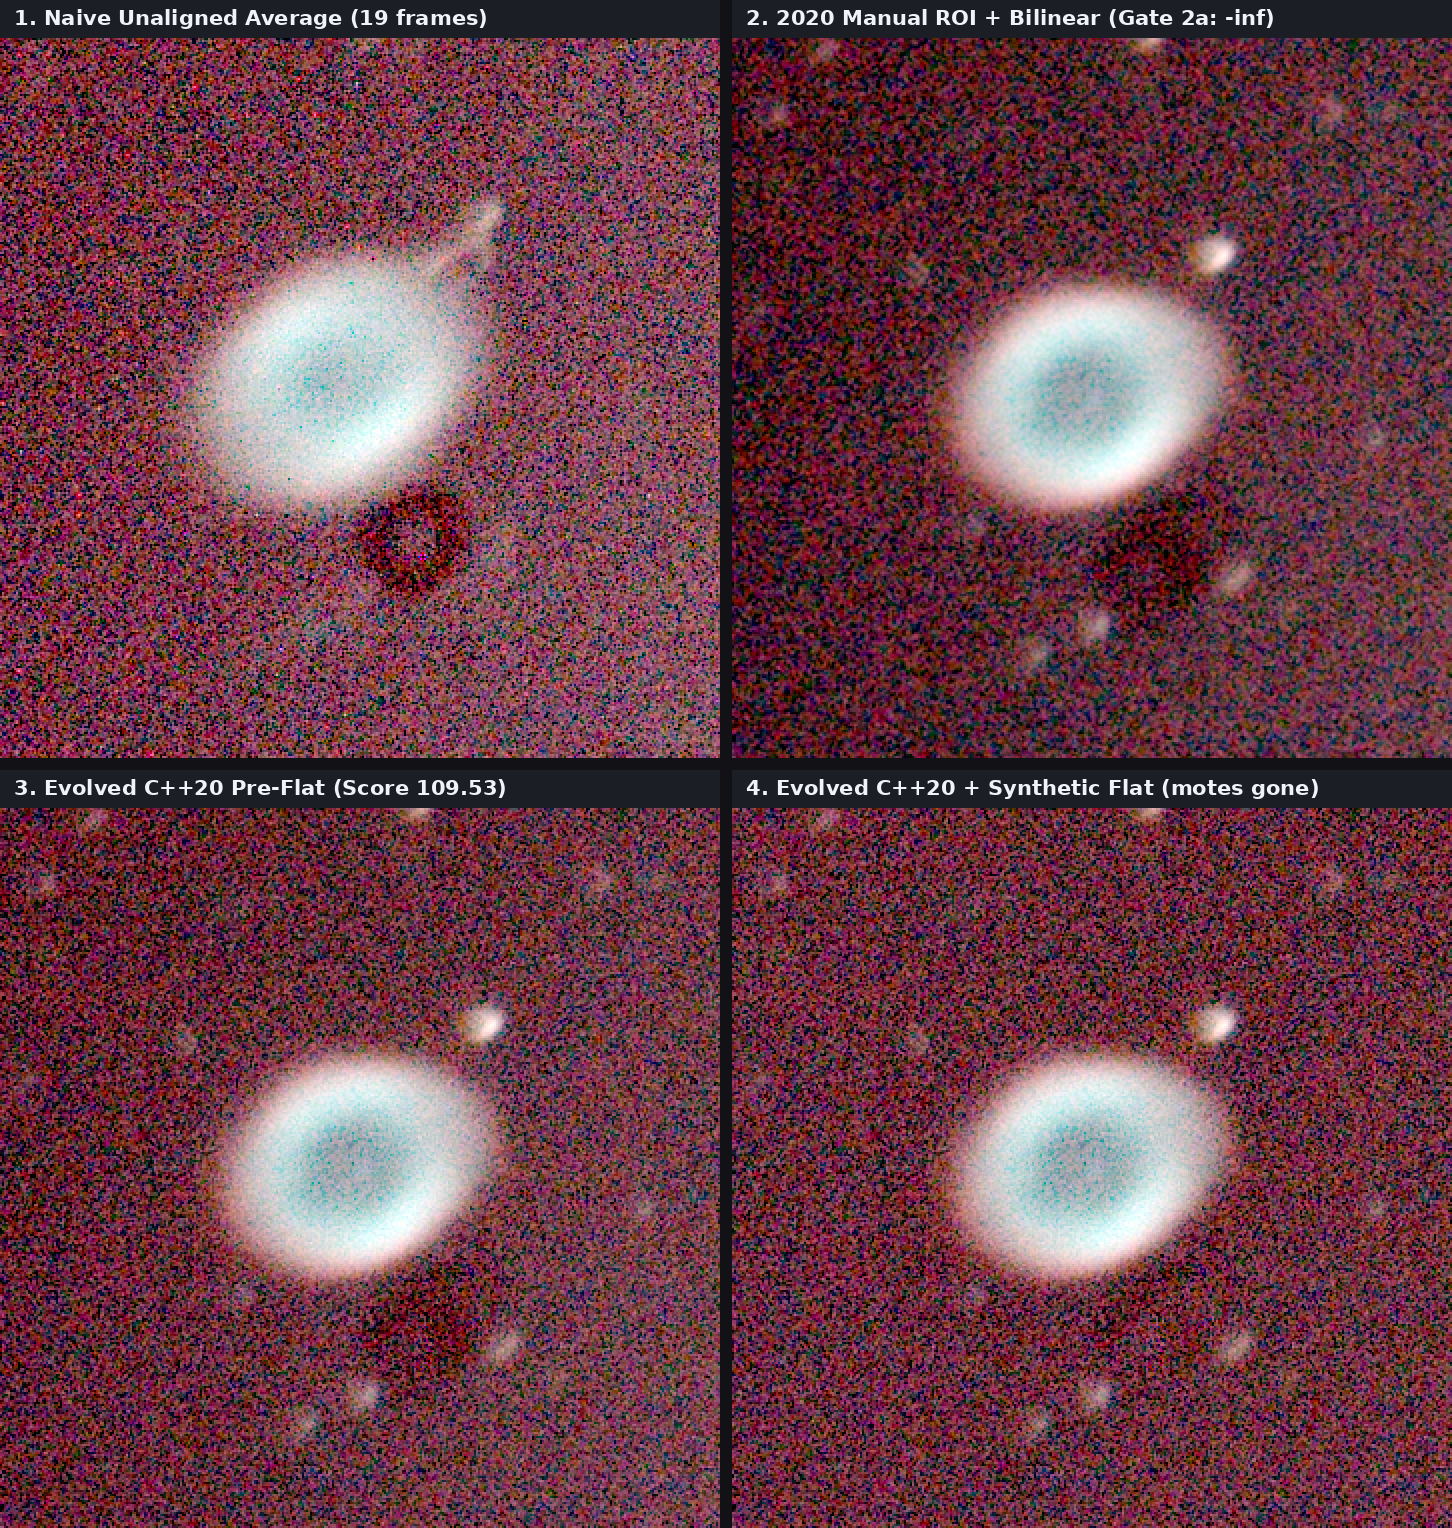
\includegraphics[width=0.46\textwidth]{ring_4stage_m57_zoom.png}
  \caption{Four-stage end-to-end visual progression on the Ring Nebula (\code{ring\_set}, 19 exposures, identical per-panel \code{asinh} stretch). \textbf{Top:} full-field progression from blind unaligned average (1) through \code{iter-0-baseline} (2) and best pre-flat stack \code{b447079} (3) to the synthetic flat-field stack \code{iter\_06\_wiener\_final} (4, $7.0\times$ flatter sky, $100\%$ of $>2\%$ dust-mote area removed). \textbf{Bottom:} $360\times 360\text{\,px}$ core zoom centered on M57 at $(1577, 1312)$, illustrating the recovery of M57's crisp ionized ring structure and central white dwarf from the smeared unaligned average.}
  \label{fig:m57_4stage}
\end{figure*}

\section{C++20/OpenMP Systems Architecture, Performance \& Conclusions}
\label{sec:performance}

\subsection{Modular C++20 Architecture \& Stage-by-Stage Throughput}

The production engine in \code{cpp\_stacker/} comprises \code{3,759} lines of strict \code{-Wall -Wextra -pedantic} C++20 compiled with \code{g++ 15.2.0} (\code{-O3 -march=native -fopenmp -lraw\_r}) into a \code{331\,KiB} standalone executable with native IEEE-754 big-endian FITS, 32-bit float TIFF, 16-bit \code{asinh}-preview TIFF, and NumPy \code{.npy} v1.0 readers/writers (\code{io\_export.cpp}), plus the optional sensor-space synthetic flat-field module (\code{flat\_field.cpp}, adding only \code{1.65\,s} in \code{motes-self}/\code{full-self} mode and \code{2.57\,s} in 3-pass \code{motes-iter} mode). Table~\ref{tab:performance} summarizes stage-by-stage 16-thread OpenMP runtimes.

Notably, \textbf{registration across all 21 frames executes in \code{33\,milliseconds}} (\code{1.6\,ms/frame}), replacing the 2020 Python \code{fftconvolve} / $[-40, 40]^2$ \code{DifferenceCorrelator} bottleneck by $>10^3\times$, while full $6\times 6$ 2D Lanczos-3 warping + per-pixel iterative Winsorized Sigma Clipping over $7.72 \times 10^8$ interpolated channel samples completes in \code{22.55\,s} via a \code{4,096}-subdivision L1-cached Lanczos lookup table and zero-allocation register insertion sorts.

\subsection{Key Scientific \& Methodological Conclusions}

\begin{enumerate}
  \item \textbf{Point-Source Geometric Hashing Defeats Coherent Sensor Systematics:} Extracting background-subtracted stellar centroids ($<0.2\%$ of pixels) and matching chirality-preserved Valdes triangle invariants completely decouples astrometry from zero-lag master-dark estimation variance, optical vignetting bowls, worm-gear velocity reversals, and celestial field rotation.
  \item \textbf{Algorithmic Evolution Is Non-Commutative:} Single-frame spatial defect repair interacts nonlinearly with downstream multi-frame integration; deferring outlier rejection to orthogonal 1D temporal Winsorized Sigma Clipping unlocked pure physical sensor calibration (\code{+0.56} combined) where premature spatial repair had regressed (\code{-0.79}).
  \item \textbf{Blind Physics Referees + Isolated Red-Team Auditors Prevent Goodhart's Law:} Pairing an immutable, torture-tested photometric referee (\code{Gates 0--5}) with per-iteration independent code/telemetry auditors enables fully autonomous scientific software engineering---achieving \code{+3.51} training gain and \code{+3.44} zero-shot out-of-distribution generalization without a single image ever entering a language model context window.
  \item \textbf{Sensor-Space Synthetic Flat-Fielding Recovers Optical Transmission Without Physical Flats:} Exploiting $47\text{--}57\text{\,px}$ mount drift to separate stationary sensor-locked optical transmission $V(\bm{x}) = V_{\text{vig}}(\bm{x})\cdot V_{\text{motes}}(\bm{x})$ from moving celestial signal in sensor coordinates prior to Lanczos-3 resampling removes $32\%$ radial vignetting to $\le 1.5\%$ residual, suppresses $>93\%$ of cross-dataset dust-mote correlation blindly across targets (\code{ring\_set} $\to$ \code{andromeda\_set}), and achieves new locked-referee highs in mote-only iterative sky-model mode (\code{109.5821} / \code{115.9508}).
\end{enumerate}

\end{document}
